\section{Performance}
\label{sec:performance}

We study the separation of the $\dihiggs$ signal from the $\ttbar$ background,
achieved by the LR $P(\vecy)$ given by Eq.~(\ref{eq:memLR}),
using samples of signal and background events produced by Monte Carlo (MC) simulation.
The samples are simulated at LO and at NLO accuracy in pQCD
and are analyzed at MC-truth as well as at detector level.
The former corresponds to the case of an ideal experimental resolution, 
while the latter aims to simulate the experimental conditions characteristic for the ATLAS and CMS experiments during LHC Run $2$.
The LO and NLO $\dihiggs$ signal samples each contain about three hundred thousand events
and the LO and NLO $\ttbar$ background samples each contain about five million events.
All samples simulated at LO accuracy in pQCD are produced with the program $\textsc{MadGraph\_aMCatNLO}$ $2.2.2$,
while the samples simulated at NLO accuracy in pQCD are produced using the program $\textsc{POWHEG}$ $v2$~\cite{POWHEG1,POWHEG2,POWHEG3,POWHEGTTBAR1,POWHEGTTBAR2,POWHEGHH1,POWHEGHH2}.
The \textrm{NNPDF3.0} LO set of PDF is used for the simulation of the LO samples and the \textrm{NNPDF3.0} NLO set for the NLO samples~\cite{NNPDF1,NNPDF2,NNPDF3}.
Parton shower and hadronization processes are modeled using the program $\textsc{PYTHIA}$ $v8.2$~\cite{Sjostrand:2014zea} with the tune \textrm{CP5}~\cite{Sirunyan:2019dfx}.
All events are generated for proton-proton collisions at $\sqrt{s} = 13$~\TeV center-of-mass energy.
Events in which the electrons or muons originate from $\Pgt$ lepton decays,
\ie from the decay chains $\PW^{+} \to \Pgt^{+}\Pnu_{\Pgt} \to \Plepton^{+}\Pnu_{\Plepton}\APnu_{\Pgt}\Pnu_{\Pgt}$ or 
$\PW^{-} \to \Pgt^{-}\APnu_{\Pgt} \to \Plepton^{-}\APnu_{\Plepton}\Pnu_{\Pgt}\APnu_{\Pgt}$, are discarded.
Detector effects are simulated using the program $\textsc{DELPHES}$ $v3.5.0$~\cite{deFavereau:2013fsa} with the card for the CMS detector.
On average forty inelastic proton-proton interactions (pileup) are added to each simulated event
in order to simulate the data-taking conditions during Run $2$ of the LHC.

Jets are reconstructed using the anti-$\kt$ algorithm~\cite{Cacciari:2008gp, Cacciari:2011ma} with a distance parameter of $0.4$,
using the detector-level particle-flow objects created by $\textsc{DELPHES}$ as input.
We refer to these jets as detector-level jets.
Their energy is corrected for pileup effects using the method described in Refs.~\cite{Cacciari:2008gn, Cacciari:2007fd}
and is calibrated as function of jet $\pT$ and $\eta$, where $\eta = -\ln\tan(\theta/2)$ denotes the pseudorapidity of the jet.
The calibration is performed such that the energy of the jets that are tagged, at detector level, as originating from the hadronization of a bottom quark
on average matches the energy of the bottom quarks that result from $\PHiggs$ boson or top quark decays at the parton level.
We refer to detector-level jets that pass the $\Pbottom$-tagging criteria as $\Pbottom$-jets.
By calibrating detector-level jets to the energy of the bottom quarks at the parton level,
the calibration procedure corrects the jet energy for out-of-cone effects and for the energy carried away, on average, by the neutrinos produced in heavy-flavor decays.

The simulated $\dihiggs$ signal and $\ttbar$ background events considered in this section are required to pass event selection criteria
similar to the analysis of $\dihiggs$ production performed, in the channel $\dihiggs \to \Pbottom\APbottom\PW\PW\virt$, by the CMS collaboration during LHC Run $2$~\cite{HIG-17-006}.
The events are required to contain two electrons or muons and two $\Pbottom$-jets.
The leptons must be within the region $\abs{\eta} < 2.5$ if they are electrons and $\abs{\eta} < 2.4$ if they are muons, and are required to be isolated.
Their isolation is computed by summing the $\pT$ of detector-level particle-flow objects that are within a cone of size
$\delta R = \sqrt{(\delta\eta)^{2} + (\delta\phi)^{2}} = 0.5$ around the lepton direction, excluding the lepton itself.
The sum is corrected for the contribution of particles from pileup using the method described in Refs.~\cite{Cacciari:2008gn, Cacciari:2007fd}.
Electrons and muons are considered isolated if the pileup-corrected sum amounts to less than $0.10$ times the $\pT$ of the lepton.
The lepton of higher $\pT$ is required to have $\pT > 25$~\GeV and the lepton of lower $\pT$ must have $\pT > 15$~\GeV.
These $\pT$ thresholds are motivated by trigger requirements.
The $\Pbottom$-jets are required to satisfy the conditions $\pT > 25$~\GeV and $\abs{\eta} < 2.4$ and to be both tagged as $\Pbottom$-jets at detector level.
The $\Pbottom$-tagging criteria implemented in the $\textsc{DELPHES}$ card for the CMS detector
corresponds to the medium working-point of the ``combined secondary vertex'' $\Pbottom$-tagging algorithm published in Ref.~\cite{CMS:2012feb}.
The algorithm identifies jets originating from the hadronization of a bottom quark with an efficiency of approximately $70\%$,
for a misidentification rate for light-quark and gluon jets of about $1.5\%$~\cite{CMS:2012feb}.
Events containing more than two $\Pbottom$-tagged jets of $\pT > 25$~\GeV and $\abs{\eta} < 2.4$ are vetoed.
The latter condition rejects a small fraction of events, amounting to $7.7\%$ of the $\dihiggs$ signal and $5.1\%$ of the $\ttbar$ background,
and avoids ambiguities in choosing the correct pair of $\Pbottom$-jets 
when computing the PDs $w_{0}(\vecy)$ and $w_{1}(\vecy)$ according to Eqs.~(\ref{eq:mem_signal}) and~(\ref{eq:mem_background}).
The selection criteria are applied to generator-level leptons and jets when analyzing simulated events at MC-truth level
and to detector-level leptons and jets when analyzing simulated events at the detector level.
In case the selection criteria are applied at MC-truth level,
no isolation requirements are applied to the leptons,
the conditions $\pT > 25$~\GeV and $\abs{\eta} < 2.4$ of the jet selection are applied at the parton level, 
to the bottom quarks that are produced in the $\PHiggs$ boson or top quark decays, and no detector-level $\Pbottom$-tagging criteria are applied.

Fig.~\ref{fig:mbb} shows the distribution in $\mbb$, the mass of the two $\Pbottom$-tagged jets at detector level, 
in $\dihiggs$ signal and $\ttbar$ background events that pass the selection criteria described in the previous paragraph.
Only events in which both detector-level jets are matched, within a cone of size $\delta R = 0.3$, 
to bottom quarks that originate from either a $\PHiggs$ boson or from top quark decays, are shown in the figure.
According to the $\textsc{DELPHES}$ simulation, 
$95.0\%$ of $\dihiggs$ and $96.4\%$ of $\ttbar$ events that pass the selection criteria described in the previous paragraph fulfill this matching condition,
\ie in $5.0\%$ of selected $\dihiggs$ and $3.6\%$ of selected $\ttbar$ events one of the bottom quarks is not reconstructed as $\Pbottom$-jet at detector level
and a light quark or gluon jet is misidentified as $\Pbottom$-jet instead.
The figure shows that the jet calibration shifts the peak of the $\mbb$ distribution by about $20\%$.
After calibration, the $\mbb$ distribution in $\dihiggs$ signal events peaks close to $125$~\GeV.
The calibration also reduces the relative width, defined as the root mean square divided by the mean, of the $\mbb$ distribution in $\dihiggs$ signal events by about $20\%$.

\begin{figure}
\ifx\ver\verPreprint
\setlength{\unitlength}{1mm}
\begin{center}
\begin{picture}(160,67)(0,0)
\put(-1.0, 1.0){\mbox{\includegraphics*[height=66mm]
 {plots/mbb_calibrated_vs_uncalibrated_signal.pdf}}}
\put(80.0, 0.0){\mbox{\includegraphics*[height=67mm]
 {plots/mbb_calibrated_vs_uncalibrated_background.pdf}}}
\end{picture}
\end{center}
\fi
\ifx\ver\verPAPER
\centering
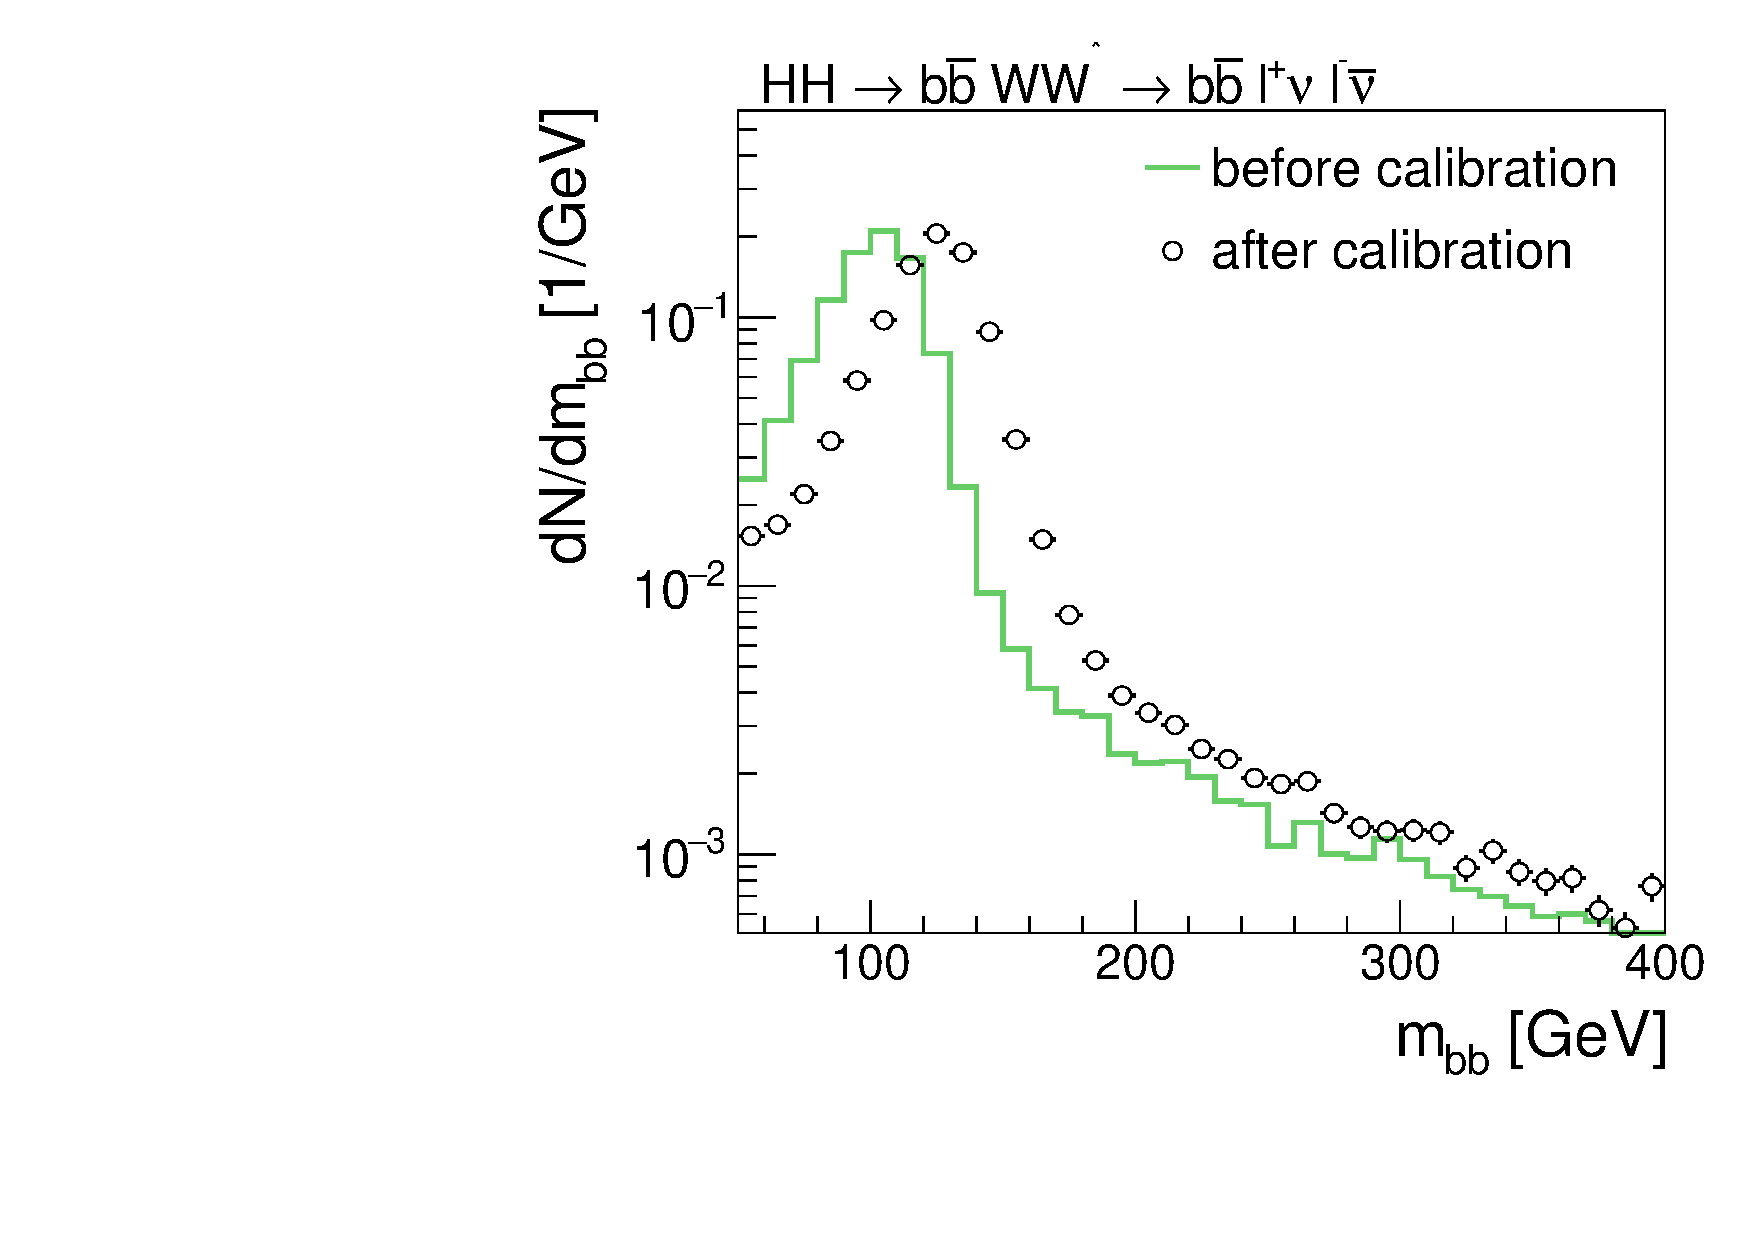
\includegraphics[width=0.48\textwidth]{plots/mbb_calibrated_vs_uncalibrated_signal.pdf}
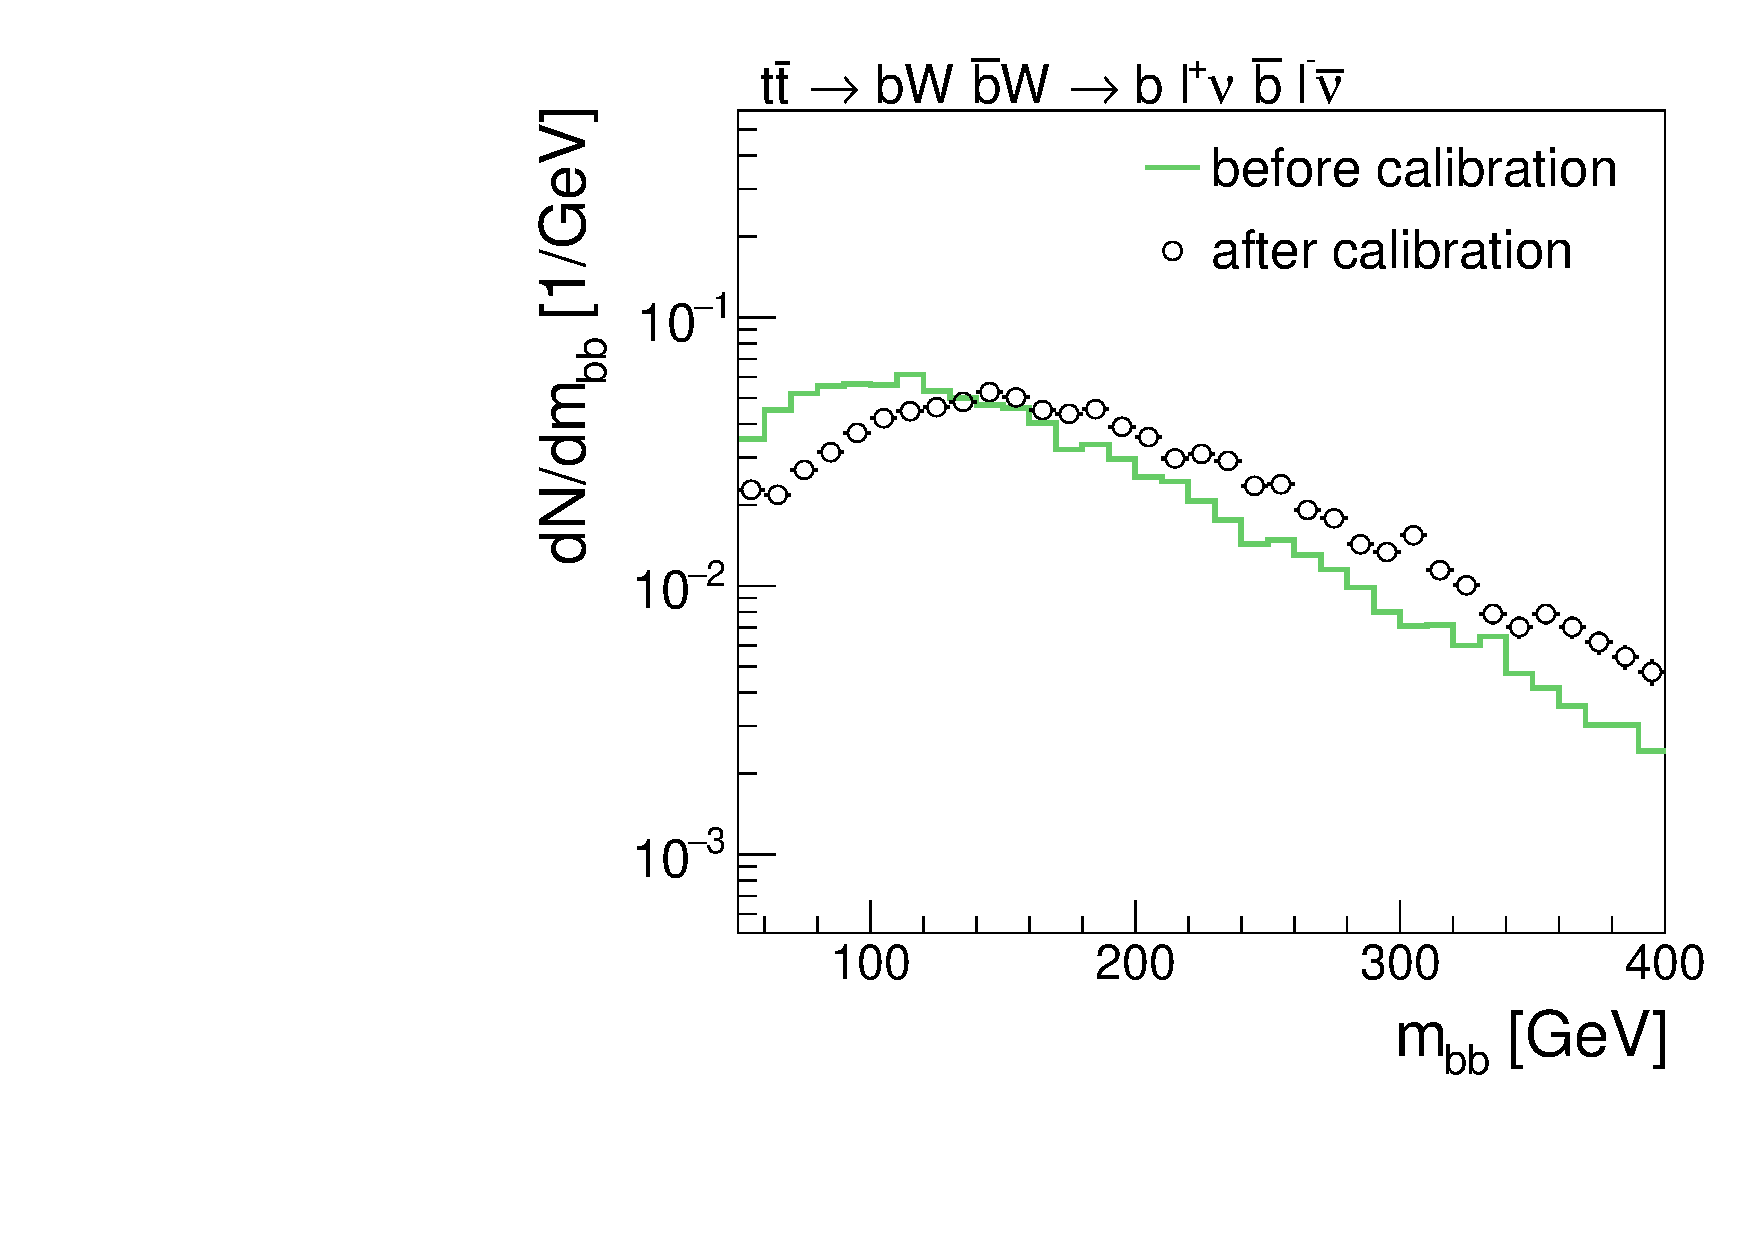
\includegraphics[width=0.48\textwidth]{plots/mbb_calibrated_vs_uncalibrated_background.pdf}
\fi
\caption{
  Distribution in $\mbb$, the mass of the two detector-level jets that are tagged as $\Pbottom$-jets,
  in $\dihiggs$ signal (left) and $\ttbar$ background (right) events before and after the jet energy calibration is applied.
}
\label{fig:mbb}
\end{figure}

In order to compute the PDs $w_{0}(\vecy)$ and $w_{1}(\vecy)$ according to Eqs.~(\ref{eq:mem_signal}) and~(\ref{eq:mem_background}),
we need to determine the TFs for the energy of $\Pbottom$-jets and for the transverse momentum components of the hadronic recoil
such that the TFs match the experimental resolution in the $\textsc{DELPHES}$ simulation.
We model the experimental resolution on the energy of $\Pbottom$-jets using a normal distribution:
\begin{linenowrapper}
\begin{equation}
W(E|\Ehat) = \frac{1}{\sqrt{2 \pi \sigma_{\Pbottom}^{2}}} \, e^{-\frac{(\pT - \pThat)^{2}}{2 \, \sigma_{\Pbottom}^{2}}} \, ,
\label{eq:resolution_b}
\end{equation}
\end{linenowrapper}
where $\pT = E \cdot \sin\theta$, $\pThat = \Ehat \cdot \sin\theta$, and $\theta$ refers to the polar angle of the jet.
The standard deviation $\sigma_{\Pbottom}$ depends on the jet energy and $\theta$.
We make the ansatz $\sigma_{\Pbottom} = k \cdot \sqrt{\Ehat \cdot \sin\theta}$ and determine the constant of proportionality $k$ such that it fits
the resolution on the energy of $\Pbottom$-jets in the $\textsc{DELPHES}$ simulation, yielding $k = 100\%$.
Our model for the jet energy resolution agrees with the resolution measured by the CMS collaboration during LHC Run $2$, shown in Fig.~3 of Ref.~\cite{JME-18-001}~\footnote{
  Our assumption that the polar angle $\theta$ of the jet is measured with negligible experimental resolution (\cf Section~\ref{sec:appendix_TF} of the appendix)
  is justified by Fig.~5 of Ref.~\cite{JME-18-001}, which shows that the resolution on $\theta$ amounts to about $0.02$ radians for jets of $\pT = 25$~\GeV and decreases for jets of higher $\pT$.}.
The hadronic recoil $\rho$ is not directly available in the $\textsc{DELPHES}$ simulation.
To determine the resolution on $\rho$, we compute the transverse momentum components of the hadronic recoil 
as function of the transverse momenta of the two leptons, the two $\Pbottom$-jets, and $\vecMET$,
using Eq.~(\ref{eq:hadRecoil_true}), with the substitutions $\pXhat^{\Pnu} + \pXhat^{\APnu} = \METxhat$ and $\pYhat^{\Pnu} + \pYhat^{\APnu} = \METyhat$, for the computation at MC-truth level 
and Eq.~(\ref{eq:hadRecoil}) for the computation at detector level.
The resolution on $\pX^{\rho}$ and $\pY^{\rho}$ in the $\textsc{DELPHES}$ simulation amounts to $32$~\GeV for the $\dihiggs$ signal and to $30$~\GeV for the $\ttbar$ background.
The resolution on the energy of $\Pbottom$-jets is small compared to the resolution on the hadronic recoil.
The resolution on the latter is thus similar to the resolution on $\vecMET$.
This similarity allows us to compare the resolutions on $\pX^{\rho}$ and $\pY^{\rho}$ in the $\textsc{DELPHES}$ simulation to the resolution on $\vecMET$
published by the ATLAS collaboration for simulated $\ttbar$ events during LHC Run $2$~\footnote{
  The CMS collaboration has not published the $\vecMET$ resolution during LHC Run $2$ specifically for $\ttbar$ events.},
which is shown in Fig.~9 of Ref.~\cite{ATLAS:2018txj} and amounts to $25$-$30$~\GeV.
We assume that the resolutions on $\pX^{\rho}$ and $\pY^{\rho}$ are uncorrelated and amount to the same for signal and background events.
Rounding the numbers for the resolution on $\pX^{\rho}$ and $\pY^{\rho}$ to one significant digit, we use:
\begin{linenowrapper}
\begin{equation}
V = \sigma_{\rho}^{2} \cdot I_{2} 
\label{eq:resolution_rho}
\end{equation}
\end{linenowrapper}
with $\sigma_{\rho} = 30$~\GeV for when computing the PDs $w_{0}(\vecy)$ and $w_{1}(\vecy)$ for $\dihiggs$ signal and $\ttbar$ background events.

We can now proceed to compute the PDs $w_{0}(\vecy)$ and $w_{1}(\vecy)$.
Distributions in $w_{0}(\vecy)$ and $w_{1}(\vecy)$ for $\dihiggs$ signal and $\ttbar$ background events are shown in Fig.~\ref{fig:probS_and_probB}.
The horizontal axis is drawn in logarithmic scale to better visualize small values of the PDs.
The PDs are computed at MC-truth and at detector level.
When computing the PDs at MC-truth level, 
we set the ``measured'' momenta of electrons and muons to their generator-level values, the ``measured'' momenta of the $\Pbottom$-jets to the momenta of the corresponding parton-level bottom quarks,
and the ``measured'' transverse momentum components of the hadronic recoil to their true values $\pXhat^{\rho}$ and $\pYhat^{\rho}$.
The latter are computed according to Eq.~(\ref{eq:hadRecoil_true}).
We also demand that both $\Pbottom$-jets are matched, within a cone of size $\delta R = 0.3$,
to bottom quarks that originate from either a $\PHiggs$ boson or from top quark decays when we compute the PDs at MC-truth level.
The same TFs, described in the previous paragraph, are used when computing the PDs $w_{0}(\vecy)$ and $w_{1}(\vecy)$ at MC-truth and at detector level.
The distributions in the PDs for the ``correct'' hypothesis ($w_{0}(\vecy)$ for signal and $w_{1}(\vecy)$ for background events)
peak close to one and fall rapidly towards smaller values, while the distributions in the PDs for the ``wrong'' hypothesis
($w_{1}(\vecy)$ for signal and $w_{0}(\vecy)$ for background events)
exhibit more pronounced tails towards small values.
Interestingly, the distributions in the PDs for the wrong hypothesis change only by a small amount between MC-truth and detector level.
The main effect of the experimental resolutions on the energy of $\Pbottom$-jets and on the transverse momentum of the hadronic recoil
as well as of the misidentification of light quark or gluon jets as $\Pbottom$-jets is to increase the tail towards small values for the distributions in the PDs for the correct hypothesis.

\begin{figure}
\ifx\ver\verPreprint
\setlength{\unitlength}{1mm}
\begin{center}
\begin{picture}(160,144)(0,0)
\put(-1.0, 78.0){\mbox{\includegraphics*[height=66mm]
 {plots/makePlotsForPaper_delphes_vs_mctruth_probS_signal.pdf}}}
\put(80.0, 78.0){\mbox{\includegraphics*[height=66mm]
 {plots/makePlotsForPaper_delphes_vs_mctruth_probS_background.pdf}}}
\put(-1.0, 0.0){\mbox{\includegraphics*[height=66mm]
 {plots/makePlotsForPaper_delphes_vs_mctruth_probB_signal.pdf}}}
\put(80.0, 0.0){\mbox{\includegraphics*[height=66mm]
 {plots/makePlotsForPaper_delphes_vs_mctruth_probB_background.pdf}}}
\end{picture}
\end{center}
\fi
\ifx\ver\verPAPER
\centering
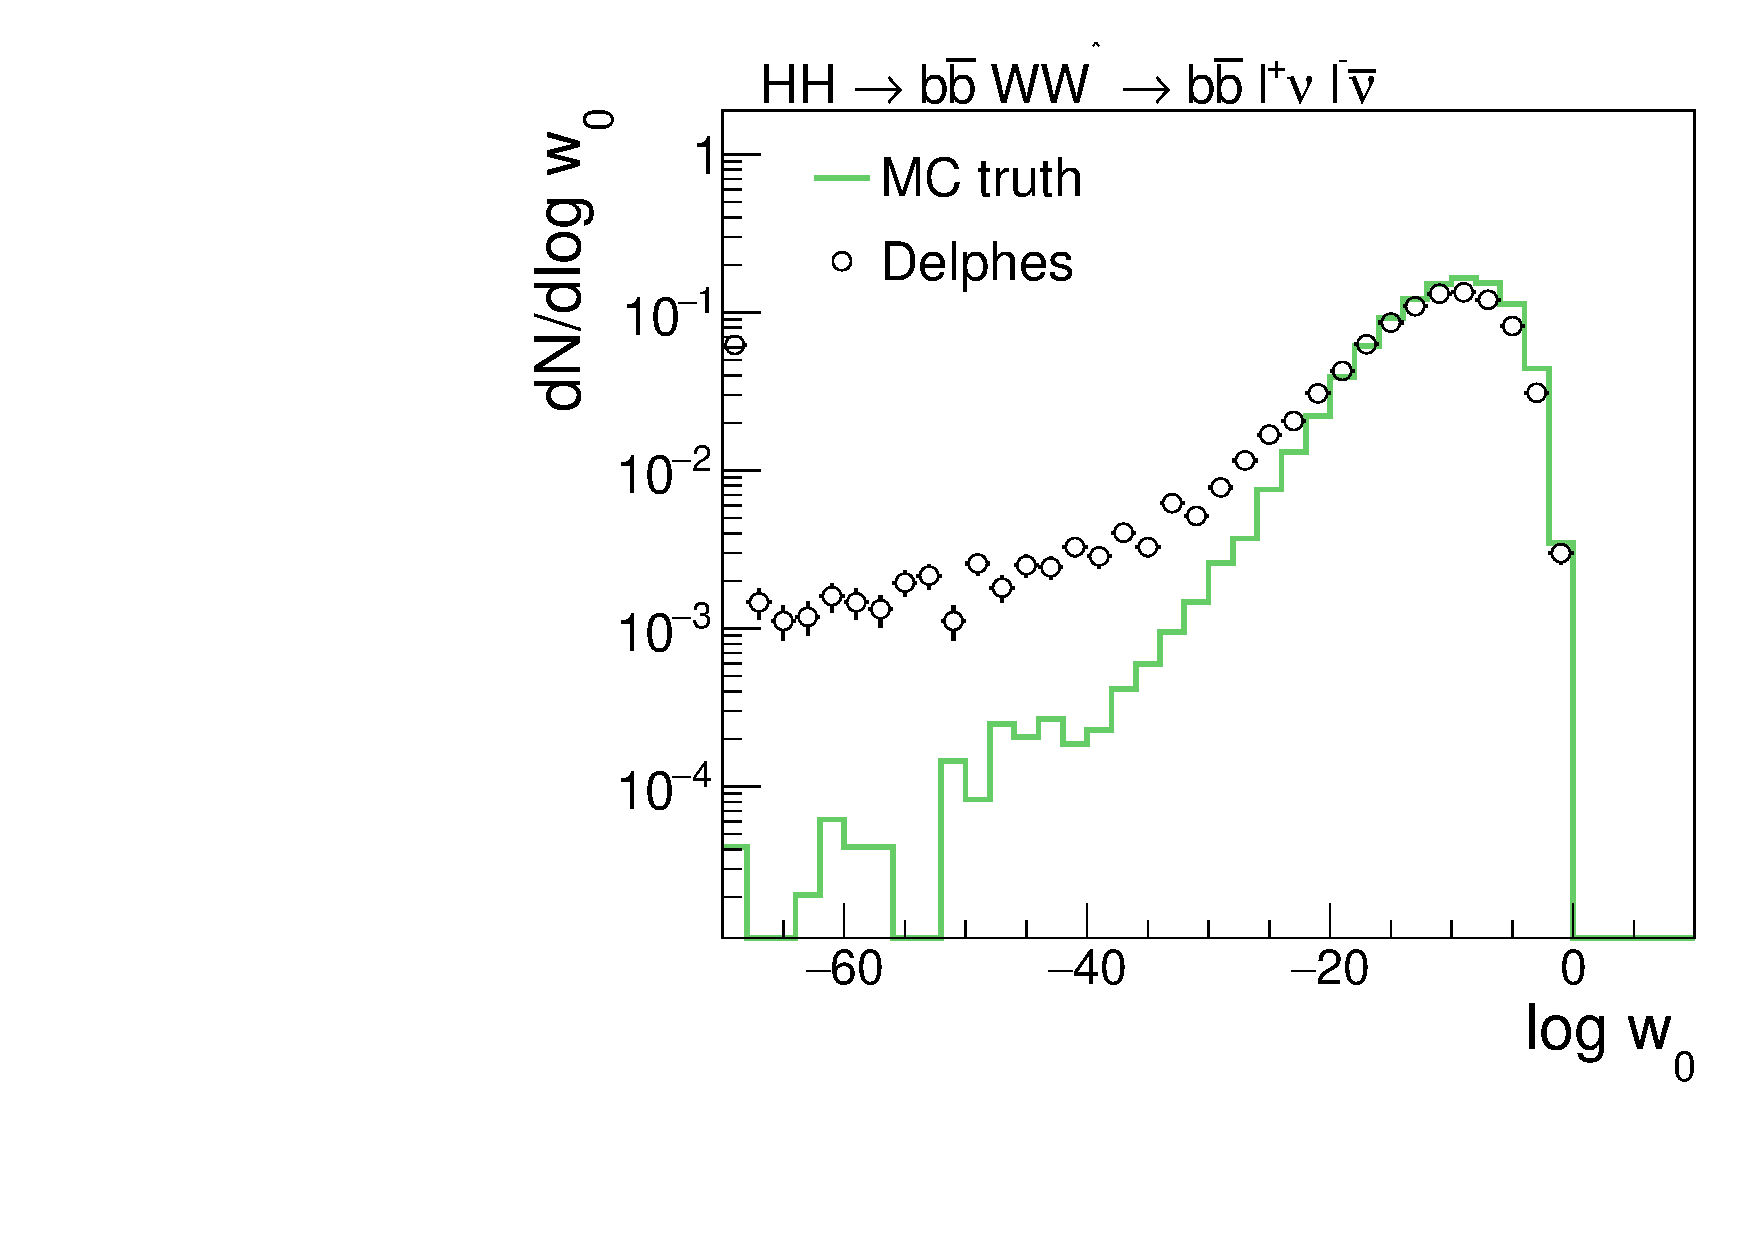
\includegraphics[width=0.48\textwidth]{plots/makePlotsForPaper_delphes_vs_mctruth_probS_signal.pdf}
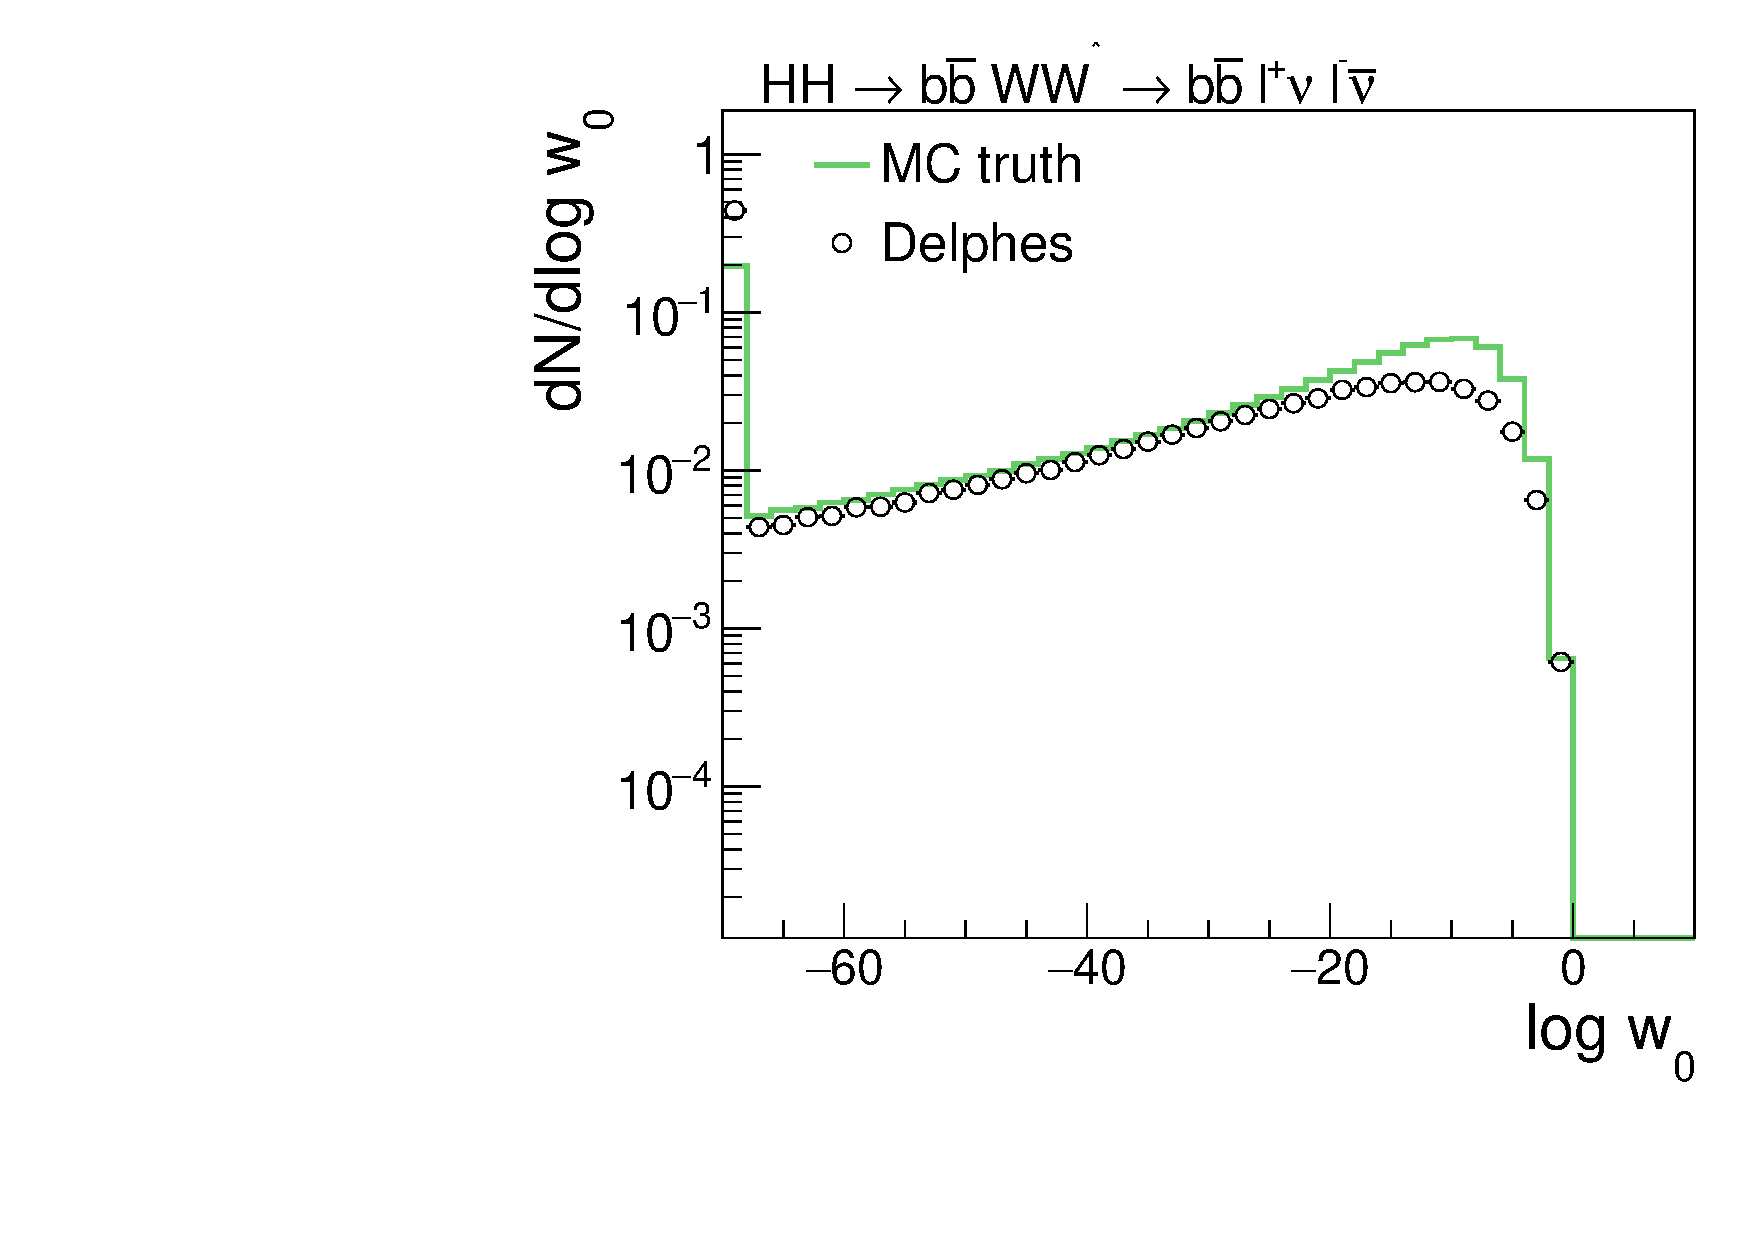
\includegraphics[width=0.48\textwidth]{plots/makePlotsForPaper_delphes_vs_mctruth_probS_background.pdf}
\hspace{0.04\textwidth}
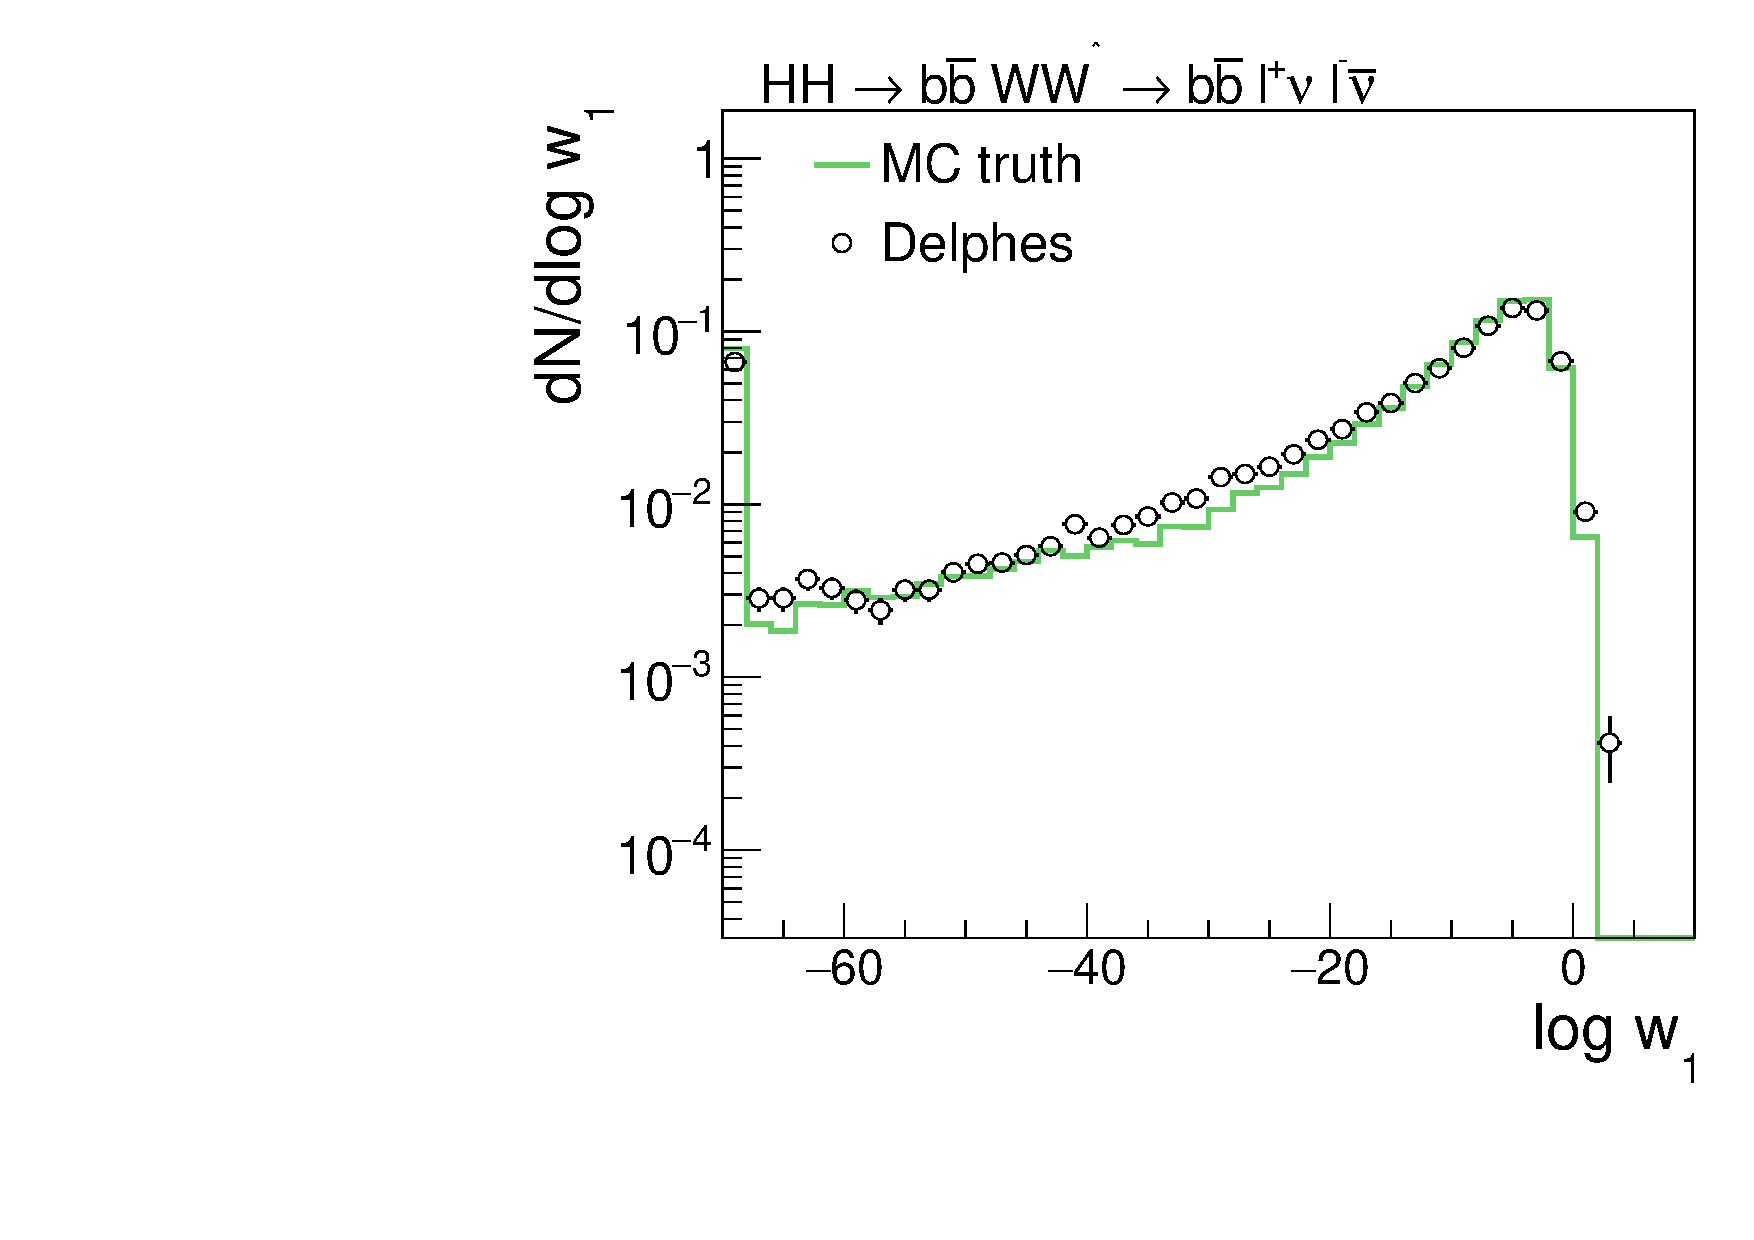
\includegraphics[width=0.48\textwidth]{plots/makePlotsForPaper_delphes_vs_mctruth_probB_signal.pdf}
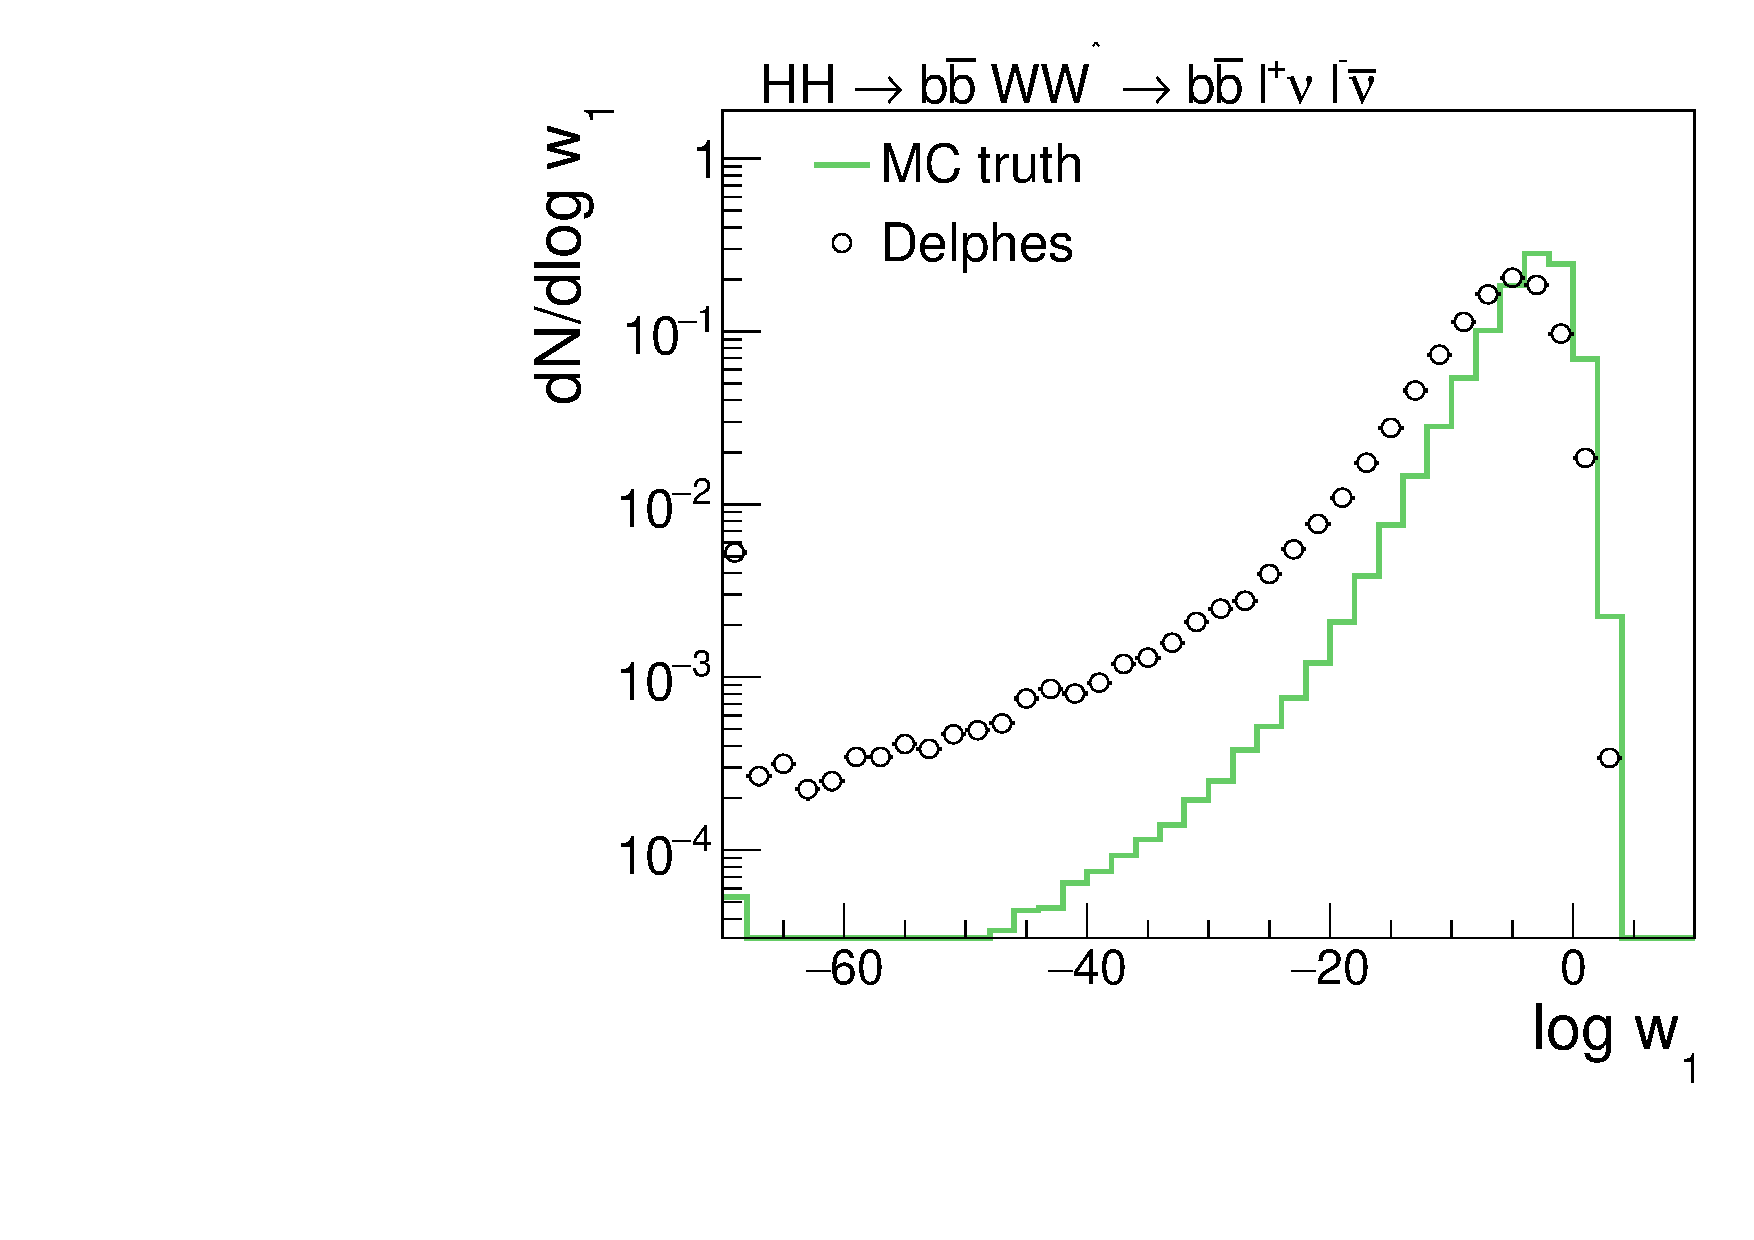
\includegraphics[width=0.48\textwidth]{plots/makePlotsForPaper_delphes_vs_mctruth_probB_background.pdf}
\fi
\caption{
  Distributions in the PDs $w_{0}(\vecy)$ (upper) and $w_{1}(\vecy)$ (lower), computed according to Eqs.~(\ref{eq:mem_signal}) and~(\ref{eq:mem_background}),
  for $\dihiggs$ signal (left) and $\ttbar$ background (right) events.
  The PDs are computed at MC-truth and at detector level.
}
\label{fig:probS_and_probB}
\end{figure}

The corresponding distributions in the LR $P(\vecy)$, computed according to Eq.~(\ref{eq:memLR}), are shown in Fig.~\ref{fig:memLR}.
Signal events are characterized by high values of $P(\vecy)$, while background events typically have low values.
The secondary peaks in the leftmost (rightmost) bin of the distribution for the $\dihiggs$ signal ($\ttbar$ background)
are due to events in which the event kinematics are atypical for signal (background) events, 
resulting in the PD for the wrong hypothesis $w_{1}(\vecy)$ ($w_{0}(\vecy)$) to be higher than the PD for the correct hypothesis $w_{0}(\vecy)$ ($w_{1}(\vecy)$).
About $4\%$ of signal ($10\%$ of background) events populate the leftmost (rightmost) bin of the distribution in case the LR $P(\vecy)$ is computed at MC-truth level.
In case the LR is computed at detector level, the fraction of $\dihiggs$ signal ($\ttbar$ background) events 
that populate the leftmost (rightmost) bin increases to $14\%$ (decreases to $7\%$).
The ``receiver-operating-characteristic'' (ROC) curves~\cite{ROCcurve} that correspond to these distributions are shown in Fig.~\ref{fig:ROC}.
The ROC curve quantifies the separation between the $\dihiggs$ signal and the $\ttbar$ background
and is obtained by varying the threshold of a cut on the LR $P(\vecy)$ and plotting the fractions of signal and background events passing the cut.
For a signal efficiency of $35\%$, the $\ttbar$ background is reduced by about three orders of magnitude, to a level of $0.09\%$, in case the LR is computed at MC-truth level.
In case the LR is computed at detector level, the $\ttbar$ background is reduced to a level of $0.26\%$.
The degradation in separation power that occurs at detector level is mainly due to 
signal events in which one of the bottom quarks originating from the $\PHiggs$ boson decay is not reconstructed as $\Pbottom$-jet at detector level
and a light quark or gluon jet is misidentified as $\Pbottom$-jet instead.
If this happens, the mass of the two detector-level jets that are reconstructed as $\Pbottom$-jets are often incompatible with $m_{\PHiggs}$.
The presence of a BW propagator in the ME $\mathcal{M}_{0}(\vecphat)$ for the signal hypothesis,
which enforces that the mass of the pair of $\Pbottom$-jets equals $m_{\PHiggs}$,
then introduces large ``pulls'' in the TF $W(E|\Ehat)$ for the $\Pbottom$-jet energy, which diminish the value of the integrand.

To better gauge the level of separation of the $\dihiggs$ signal from the $\ttbar$ background presented in Fig.~\ref{fig:ROC},
we compute signal efficiencies and background rates that one would obtain by cutting on the mass, $\mbb$, of the $\Pbottom$-jet pair, shown in Fig.~\ref{fig:mbb}, for comparison.
The observable $\mbb$ is presumably one of the most powerful single observables to separate the $\dihiggs$ signal from the $\ttbar$ background.
Fitting the peak of the distribution in the mass of the $\Pbottom$-jet pair in $\dihiggs$ signal events, obtained after the jet energy calibration is applied,
with a normal distribution yields a mean of $123$~\GeV and a standard deviation of $20$~\GeV.
Requiring events to have a value of $\mbb$ within $1$ ($2$) standard deviations around the mean
selects $78\%$ ($89\%$) of the $\dihiggs$ signal and $27\%$ ($43\%$) of the $\ttbar$ background.
Compared to the cut on $\mbb$,
the LR $P(\vecy)$ allows for a significantly higher reduction in the rate of $\ttbar$ background
by exploiting the full difference in event kinematics between the $\dihiggs$ signal and the $\ttbar$ background.

We remark that the misidentification of hadrons as leptons is not simulated in $\textsc{DELPHES}$ and hence not accounted for in the detector-level ROC curve shown in Fig.~\ref{fig:ROC}.
Based on the analysis of $\dihiggs$ production performed in the decay channel $\Pbottom\APbottom\PW\PW\virt$ by the CMS collaboration during LHC Run $2$~\cite{HIG-17-006},
which found the background arising from the misidentification of hadrons as leptons to be negligible,
we expect the misidentification of hadrons as leptons to have at most a small effect on the ROC curve.

\begin{figure}
\ifx\ver\verPreprint
\setlength{\unitlength}{1mm}
\begin{center}
\begin{picture}(160,66)(0,0)
\put(-1.0, 0.0){\mbox{\includegraphics*[height=66mm]
 {plots/makePlotsForPaper_delphes_vs_mctruth_memLR_signal.pdf}}}
\put(80.0, 0.0){\mbox{\includegraphics*[height=66mm]
 {plots/makePlotsForPaper_delphes_vs_mctruth_memLR_background.pdf}}}
\end{picture}
\end{center}
\fi
\ifx\ver\verPAPER
\centering
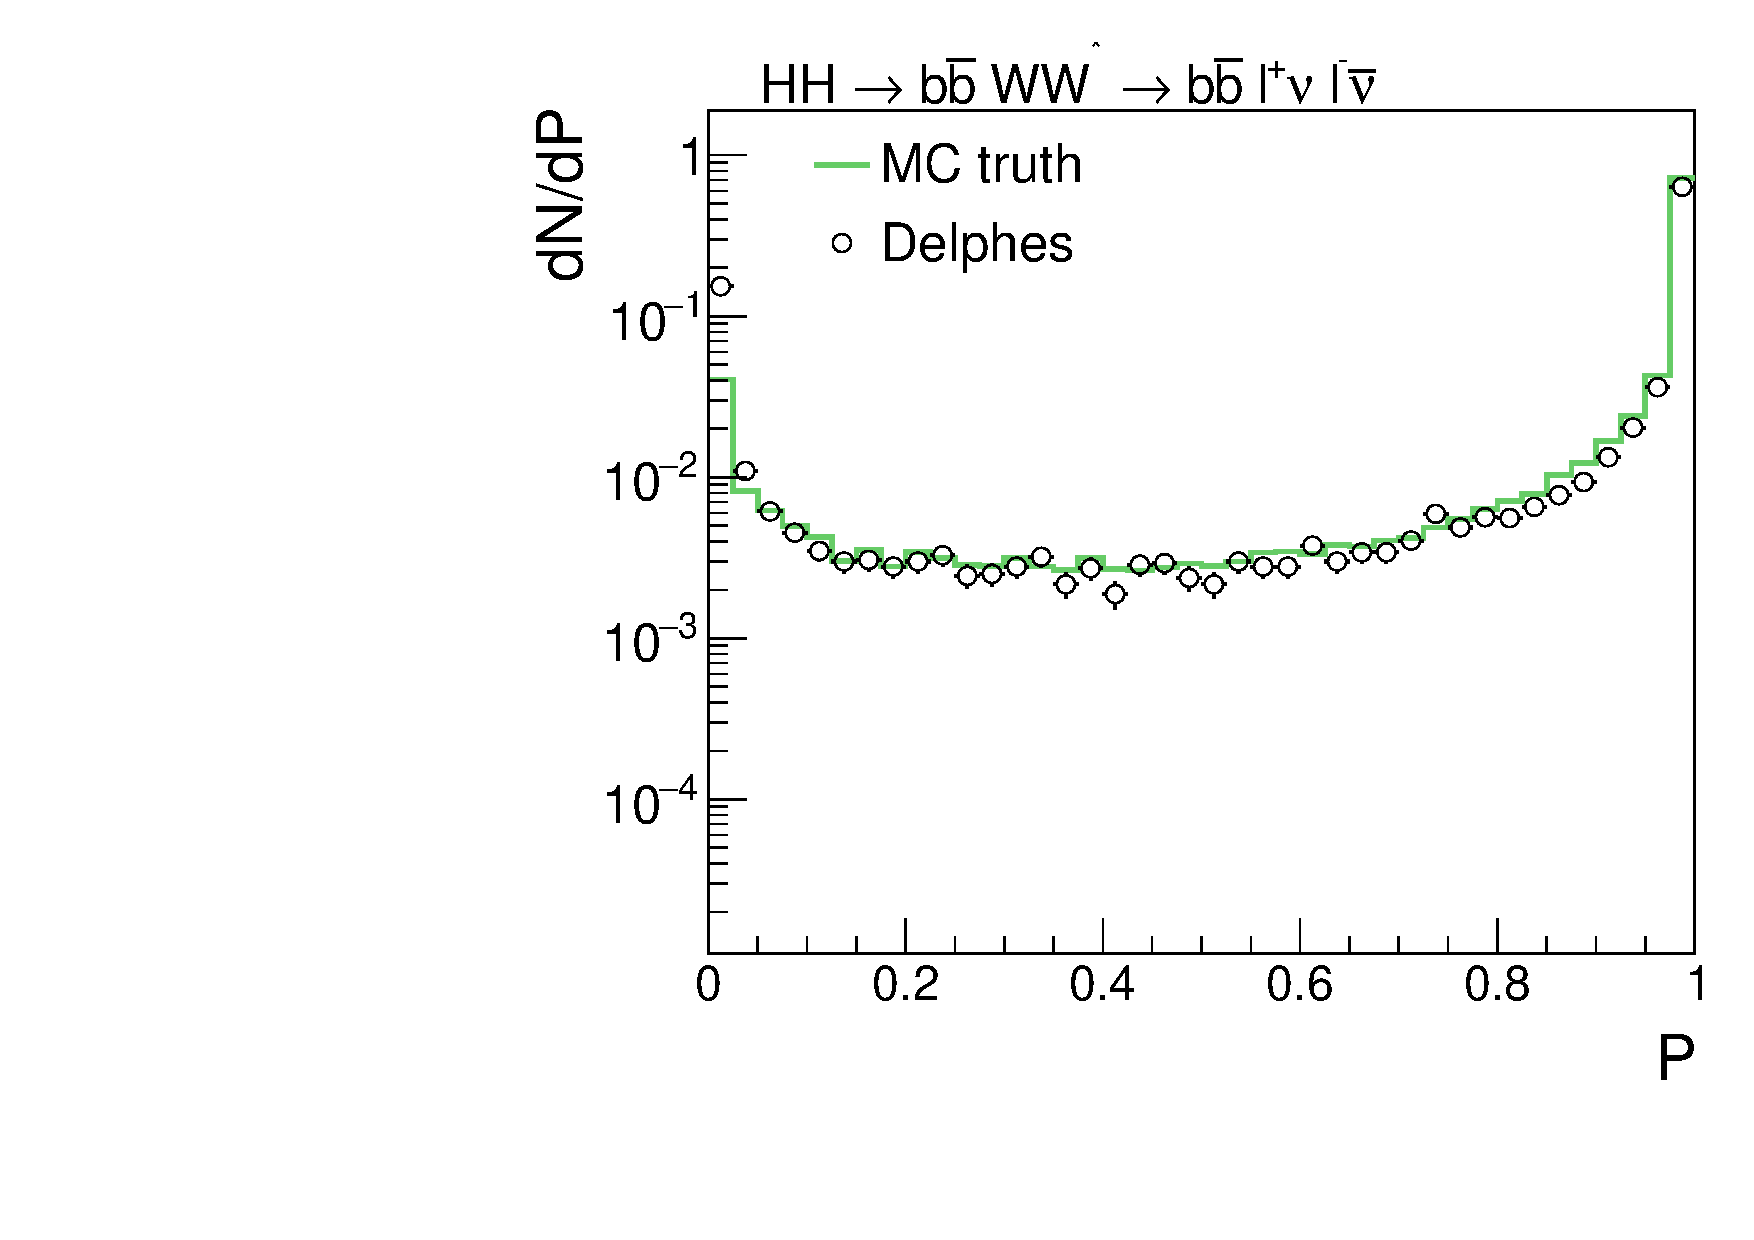
\includegraphics[width=0.48\textwidth]{plots/makePlotsForPaper_delphes_vs_mctruth_memLR_signal.pdf}
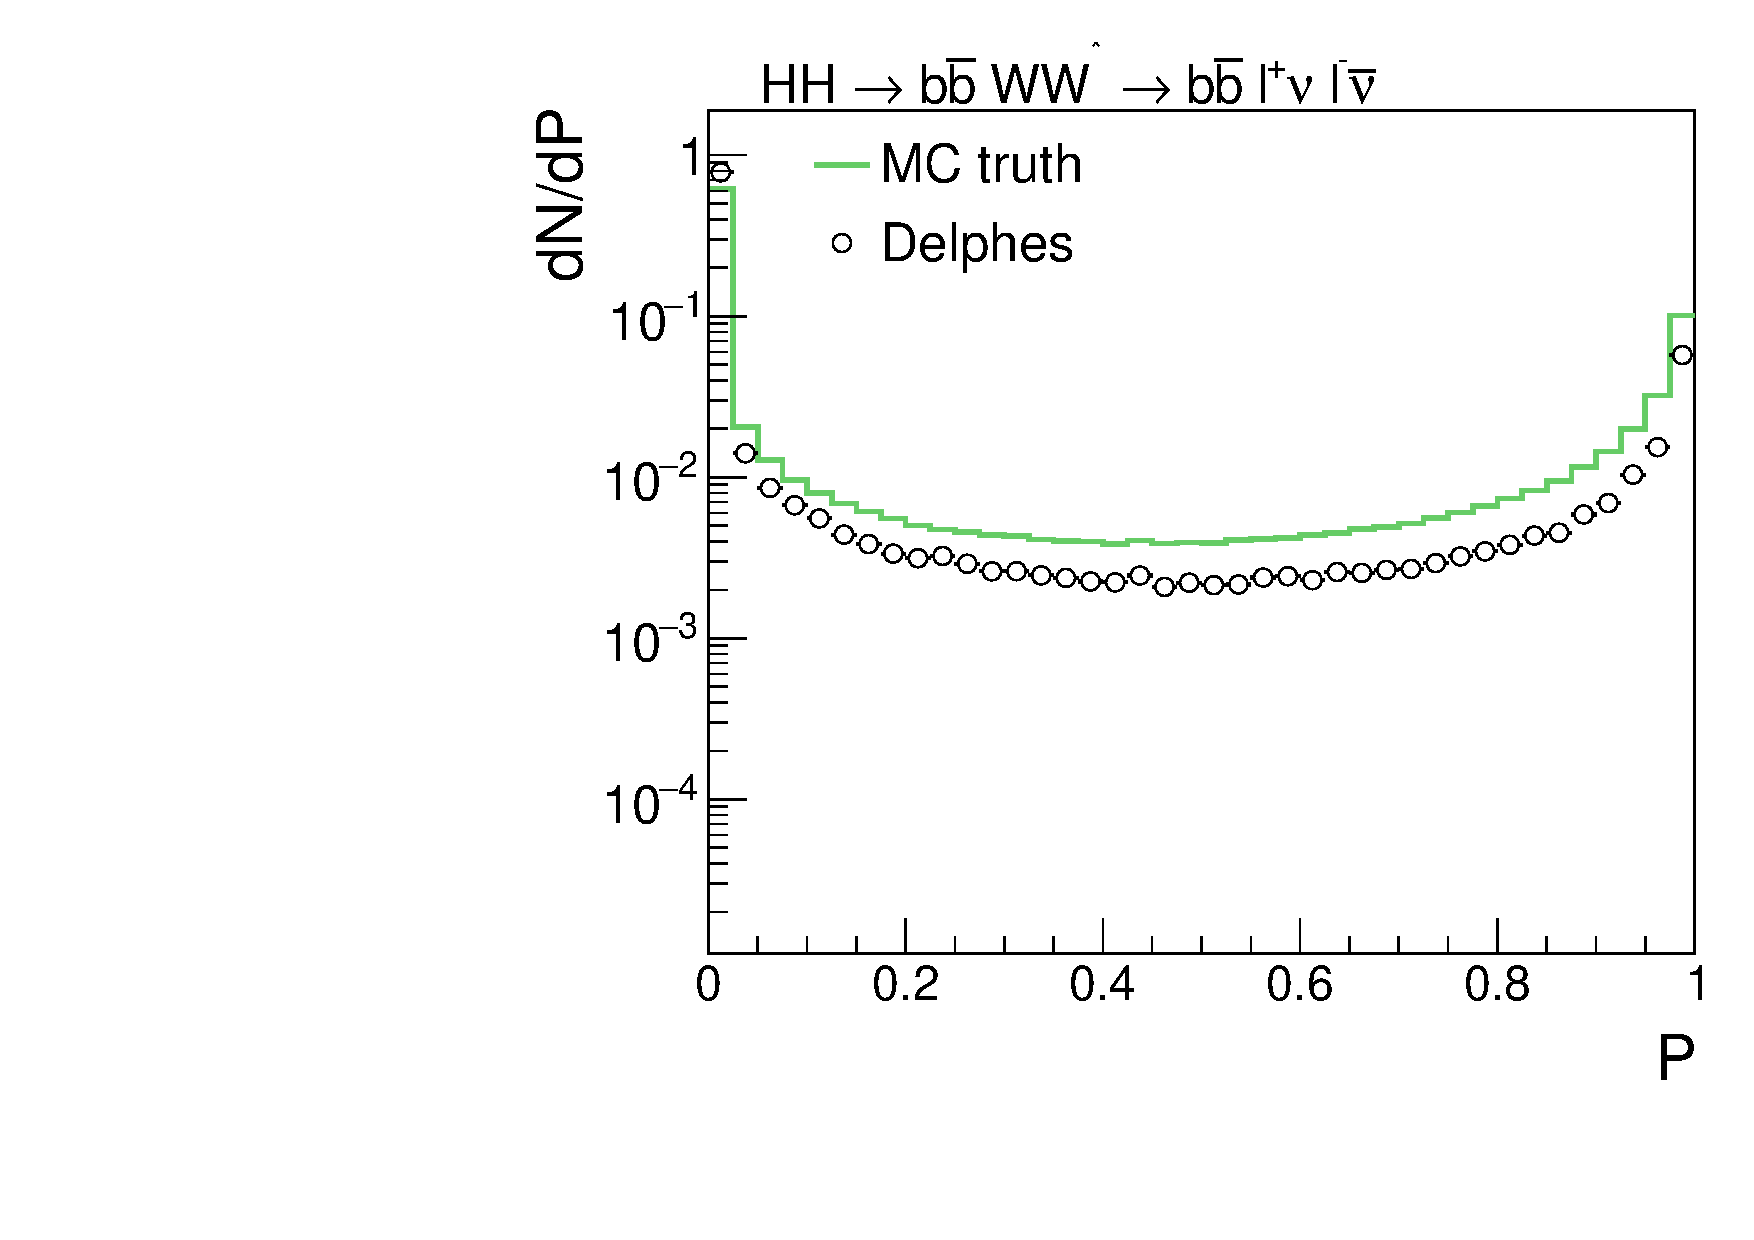
\includegraphics[width=0.48\textwidth]{plots/makePlotsForPaper_delphes_vs_mctruth_memLR_background.pdf}
\fi
\caption{
  Distributions in the LR $P(\vecy)$, computed according to Eq.~(\ref{eq:memLR}),
  for $\dihiggs$ signal (left) and $\ttbar$ background (right) events.
  The LR $P(\vecy)$ is computed using the PDs $w_{0}(\vecy)$ and $w_{1}(\vecy)$ shown in Fig.~\ref{fig:probS_and_probB} as input
  and is computed at MC-truth and at detector level.
}
\label{fig:memLR}
\end{figure}

\begin{figure}
\ifx\ver\verPreprint
\setlength{\unitlength}{1mm}
\begin{center}
\begin{picture}(160,67)(0,0)
\put(39.5, 0.0){\mbox{\includegraphics*[height=67mm]
 {plots/makePlotsForPaper_delphes_vs_mctruth_ROC.pdf}}}
\end{picture}
\end{center}
\fi
\ifx\ver\verPAPER
\centering
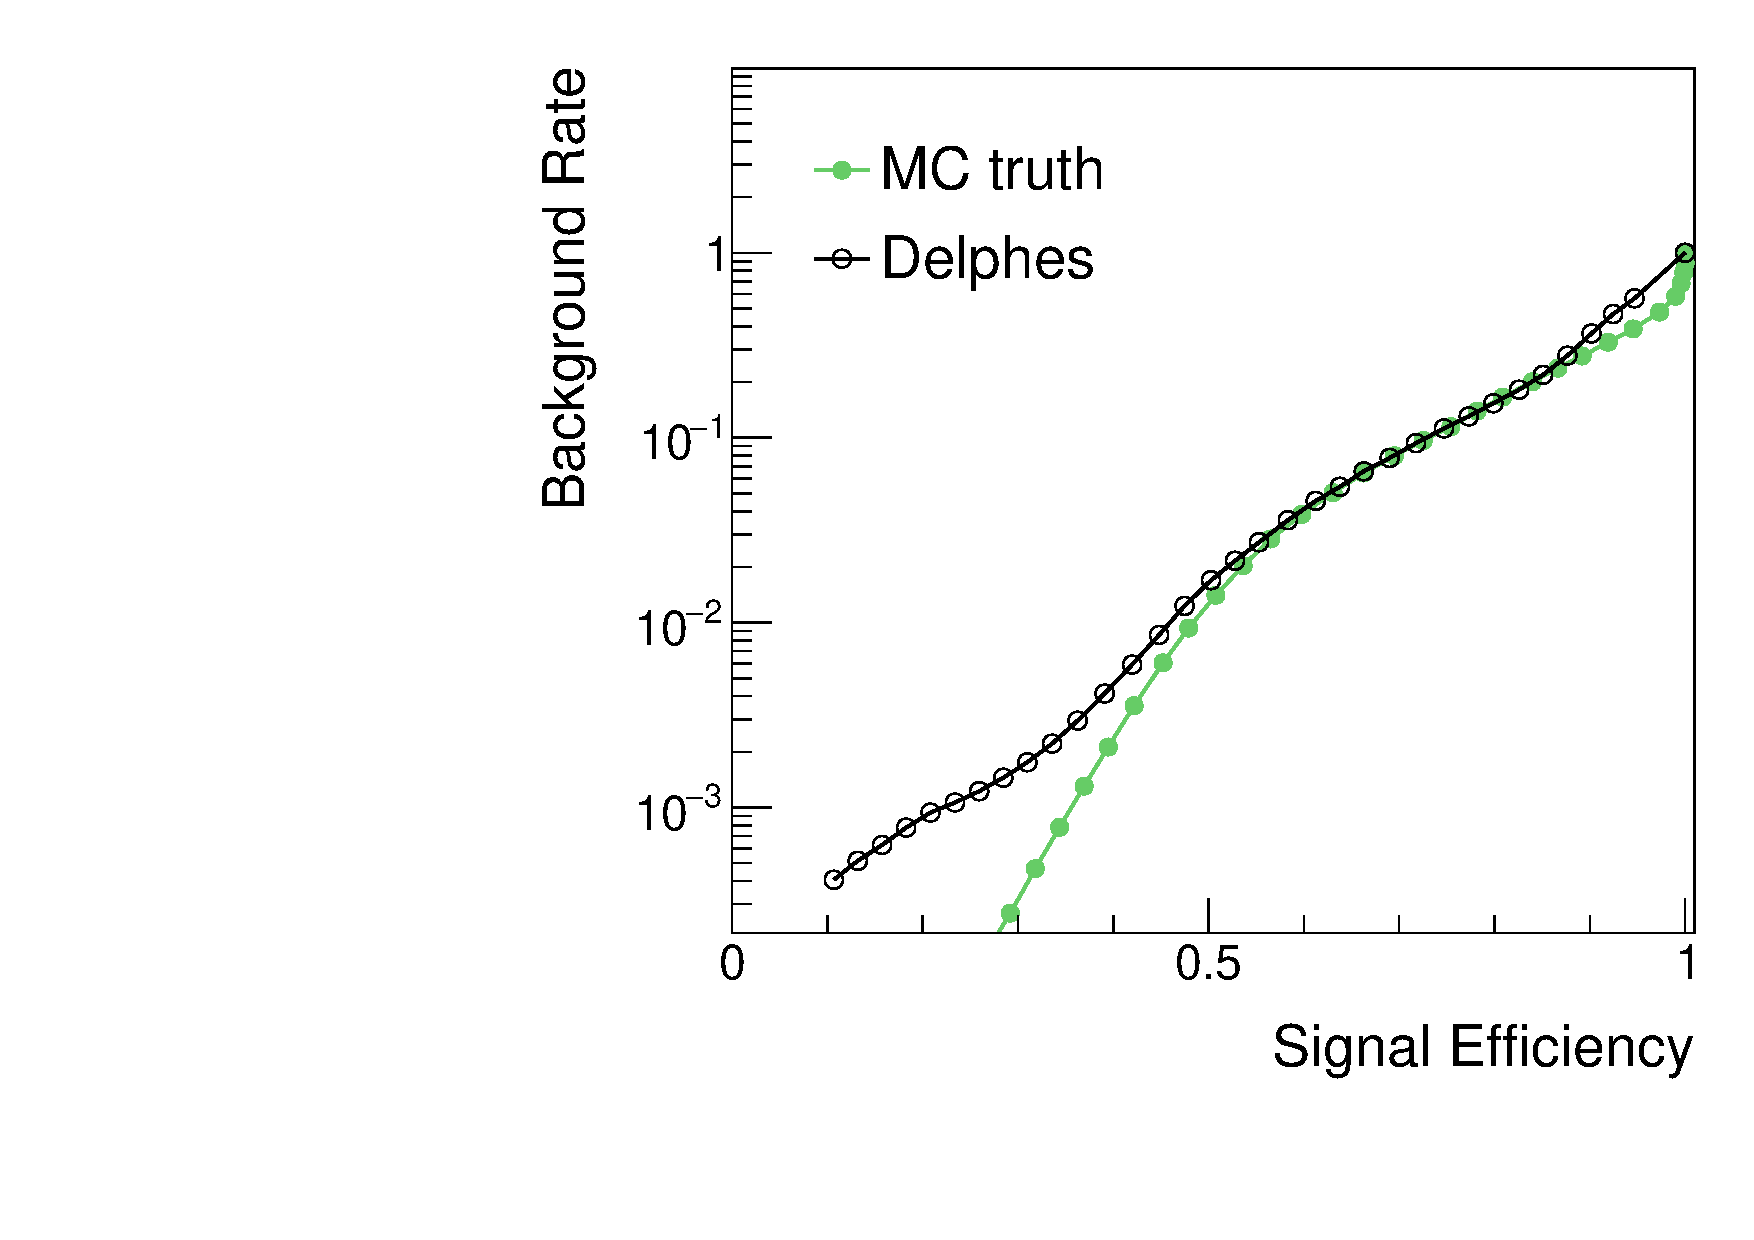
\includegraphics[width=0.57\textwidth]{plots/makePlotsForPaper_delphes_vs_mctruth_ROC.pdf}
\fi
\caption{
  Graphs of background rate versus signal efficiency (``ROC curve''), at MC-truth and at detector level,
  obtained by varying the threshold of a cut applied on the distributions in the LR $P(\vecy)$ shown in Fig.~\ref{fig:memLR}.
}
\label{fig:ROC}
\end{figure}

We conclude this section on the performance of the MEM with a study of the effect of using ME of LO when computing the weights $w_{0}(\vecy)$ and $w_{1}(\vecy)$ 
by means of Eqs.~(\ref{eq:mem_signal}) and~(\ref{eq:mem_background}) and with a discussion of the computing-time requirements of the MEM.

Unfortunately, we cannot compare the performance of the MEM
for the case of using ME generated at LO versus ME generated at NLO in Eqs.~(\ref{eq:mem_signal}) and~(\ref{eq:mem_background}) directly,
because the program $\textsc{MadGraph\_aMCatNLO}$ does not support the generation of code for NLO ME at present
and also because the usage of NLO ME in the MEM would increase the computing-time requirements by $1$-$2$ orders of magnitude.
Instead, we use ME generated at LO accuracy in Eqs.~(\ref{eq:mem_signal}) and~(\ref{eq:mem_background}) 
and compare the resulting performance in separating the $\dihiggs$ signal from the $\ttbar$ background
for MC samples simulated at LO and at NLO accuracy in pQCD.
The NLO samples are expected to provide the more accurate modelling of real data and the LO samples are taken as a (more or less precise) approximation.
We take the difference in performance achieved by the MEM on the MC samples simulated at LO and at NLO accuracy
as an estimate for the loss in discrimination power that results from our choice of using LO ME and ignoring the effects of higher orders in the MEM.
Distributions in the LR $P(\vecy)$ computed for $\dihiggs$ signal and $\ttbar$ background events simulated at LO and at NLO accuracy in pQCD 
are shown in Fig.~\ref{fig:memLR_LO_vs_NLO}. The events are analyzed at MC-truth level.
The corresponding ROC curve is presented in Fig.~\ref{fig:ROC_LO_vs_NLO}.
The usage of LO ME causes a moderate loss in the separation of the $\dihiggs$ signal from the $\ttbar$ background,
amounting to a few percent loss in signal efficiency (for the same background rate).
We conclude from these figures that the usage of LO ME represents a viable approximation.

\begin{figure}
\ifx\ver\verPreprint
\setlength{\unitlength}{1mm}
\begin{center}
\begin{picture}(160,78)(0,0)
\put(0.0, 0.0){\mbox{\includegraphics*[height=78mm]
 {plots/hh_bbwwMEM_dilepton_lo_vs_nlo_memLR_signal.pdf}}}
\put(81.0, 0.0){\mbox{\includegraphics*[height=78mm]
 {plots/hh_bbwwMEM_dilepton_lo_vs_nlo_memLR_background.pdf}}}
\end{picture}
\end{center}
\fi
\ifx\ver\verPAPER
\centering
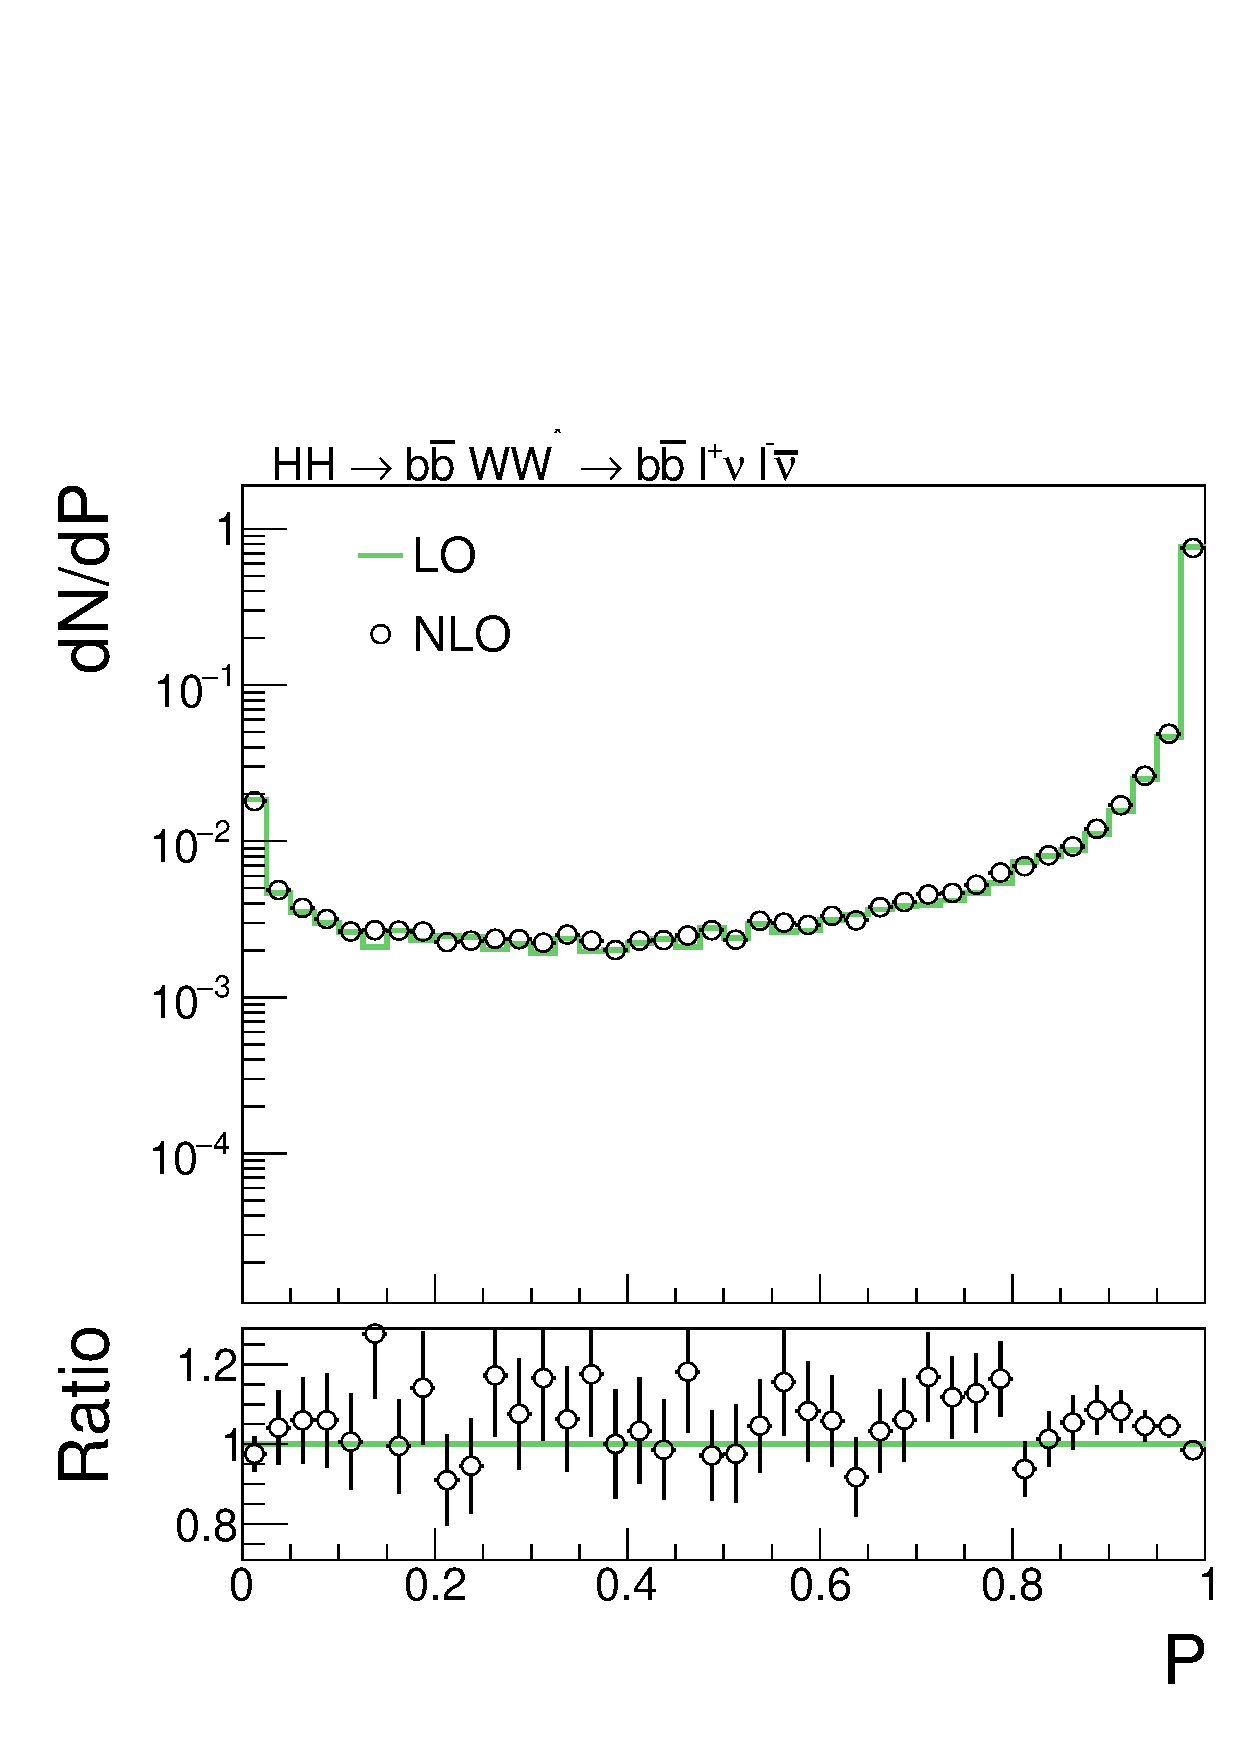
\includegraphics[width=0.48\textwidth]{plots/hh_bbwwMEM_dilepton_lo_vs_nlo_memLR_signal.pdf}
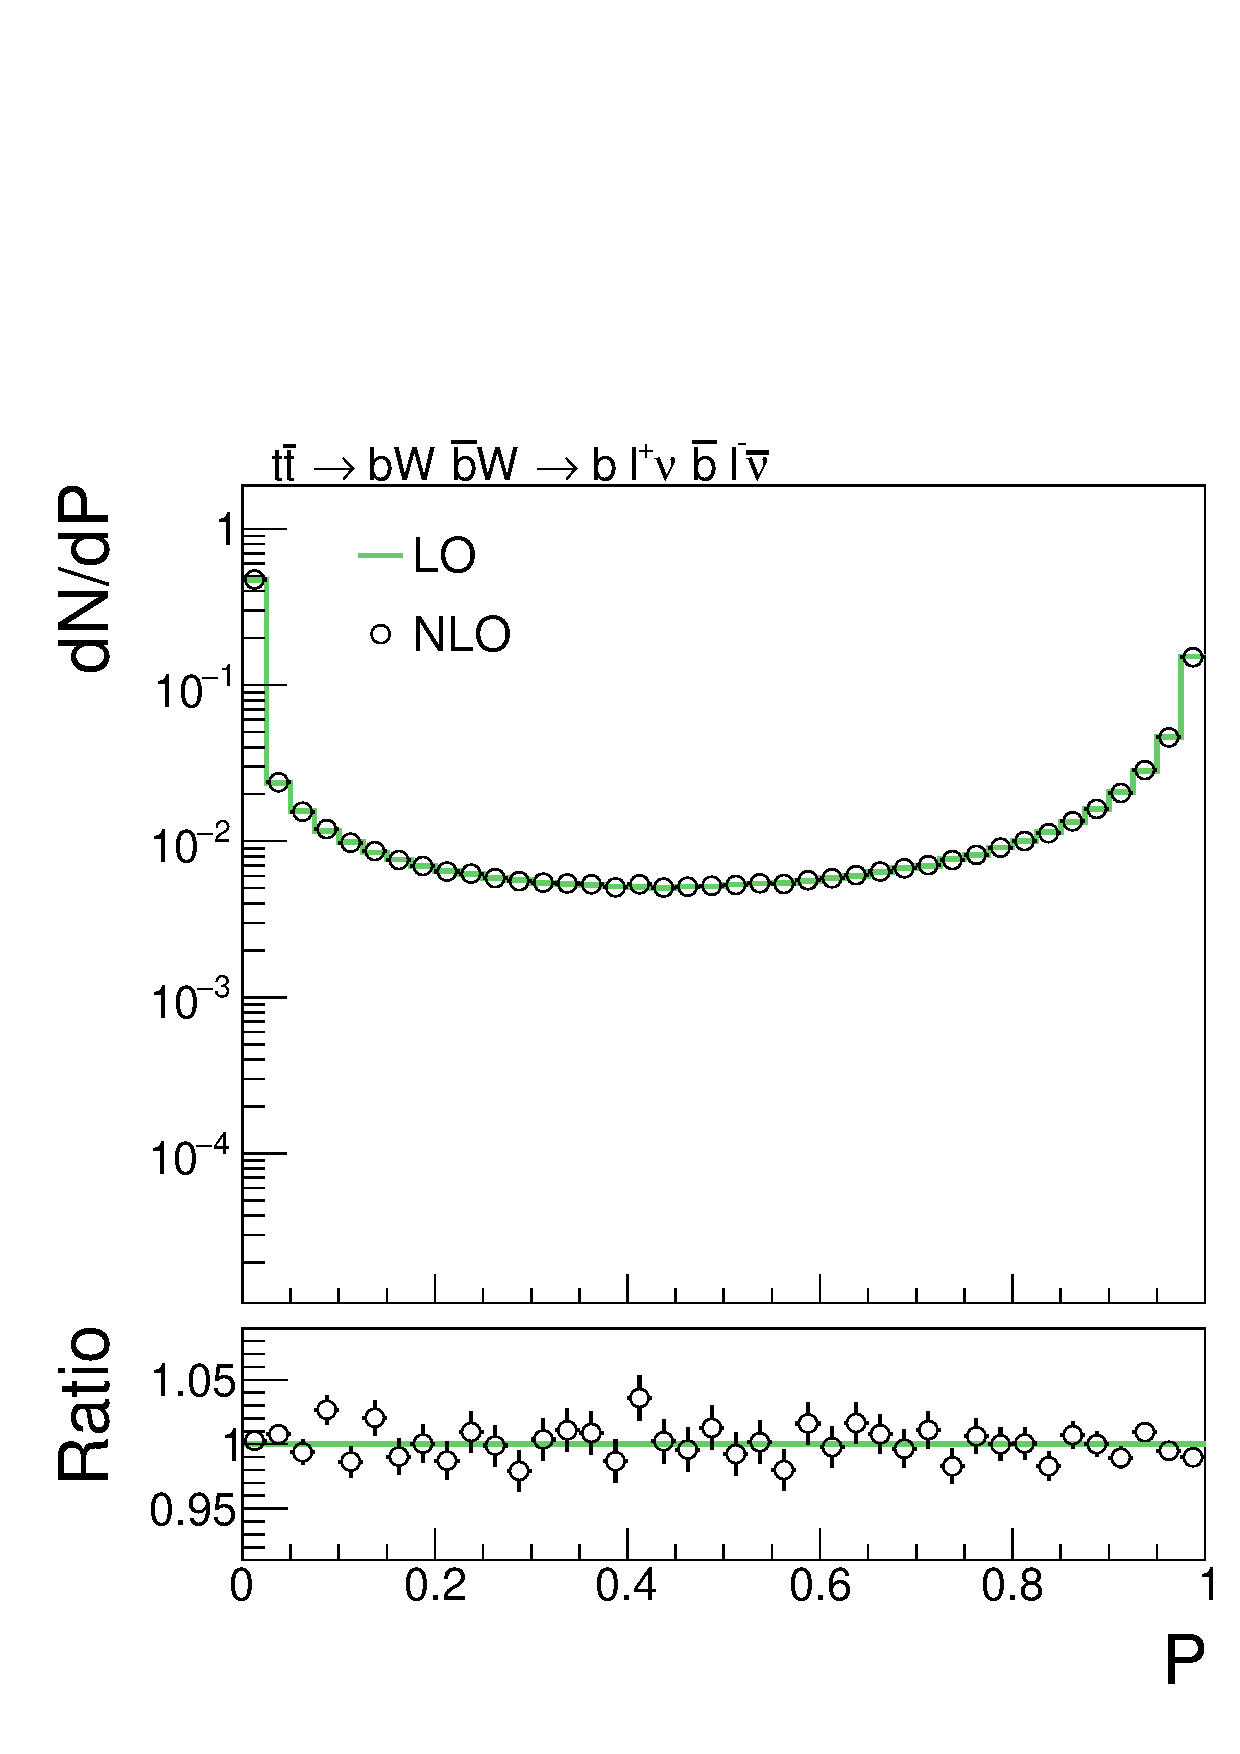
\includegraphics[width=0.48\textwidth]{plots/hh_bbwwMEM_dilepton_lo_vs_nlo_memLR_background.pdf}
\fi
\caption{
  Distribution in the LR $P(\vecy)$ 
  for $\dihiggs$ signal (left) and $\ttbar$ background (right) events
  simulated at LO and at NLO accuracy in pQCD.
  The likelihood ratios are computed at MC-truth level.
}
\label{fig:memLR_LO_vs_NLO}
\end{figure}

\begin{figure}
\ifx\ver\verPreprint
\setlength{\unitlength}{1mm}
\begin{center}
\begin{picture}(160,67)(0,0)
\put(39.5, 0.0){\mbox{\includegraphics*[height=67mm]
 {plots/hh_bbwwMEM_dilepton_lo_vs_nlo_ROC.pdf}}}
\end{picture}
\end{center}
\fi
\ifx\ver\verPAPER
\centering
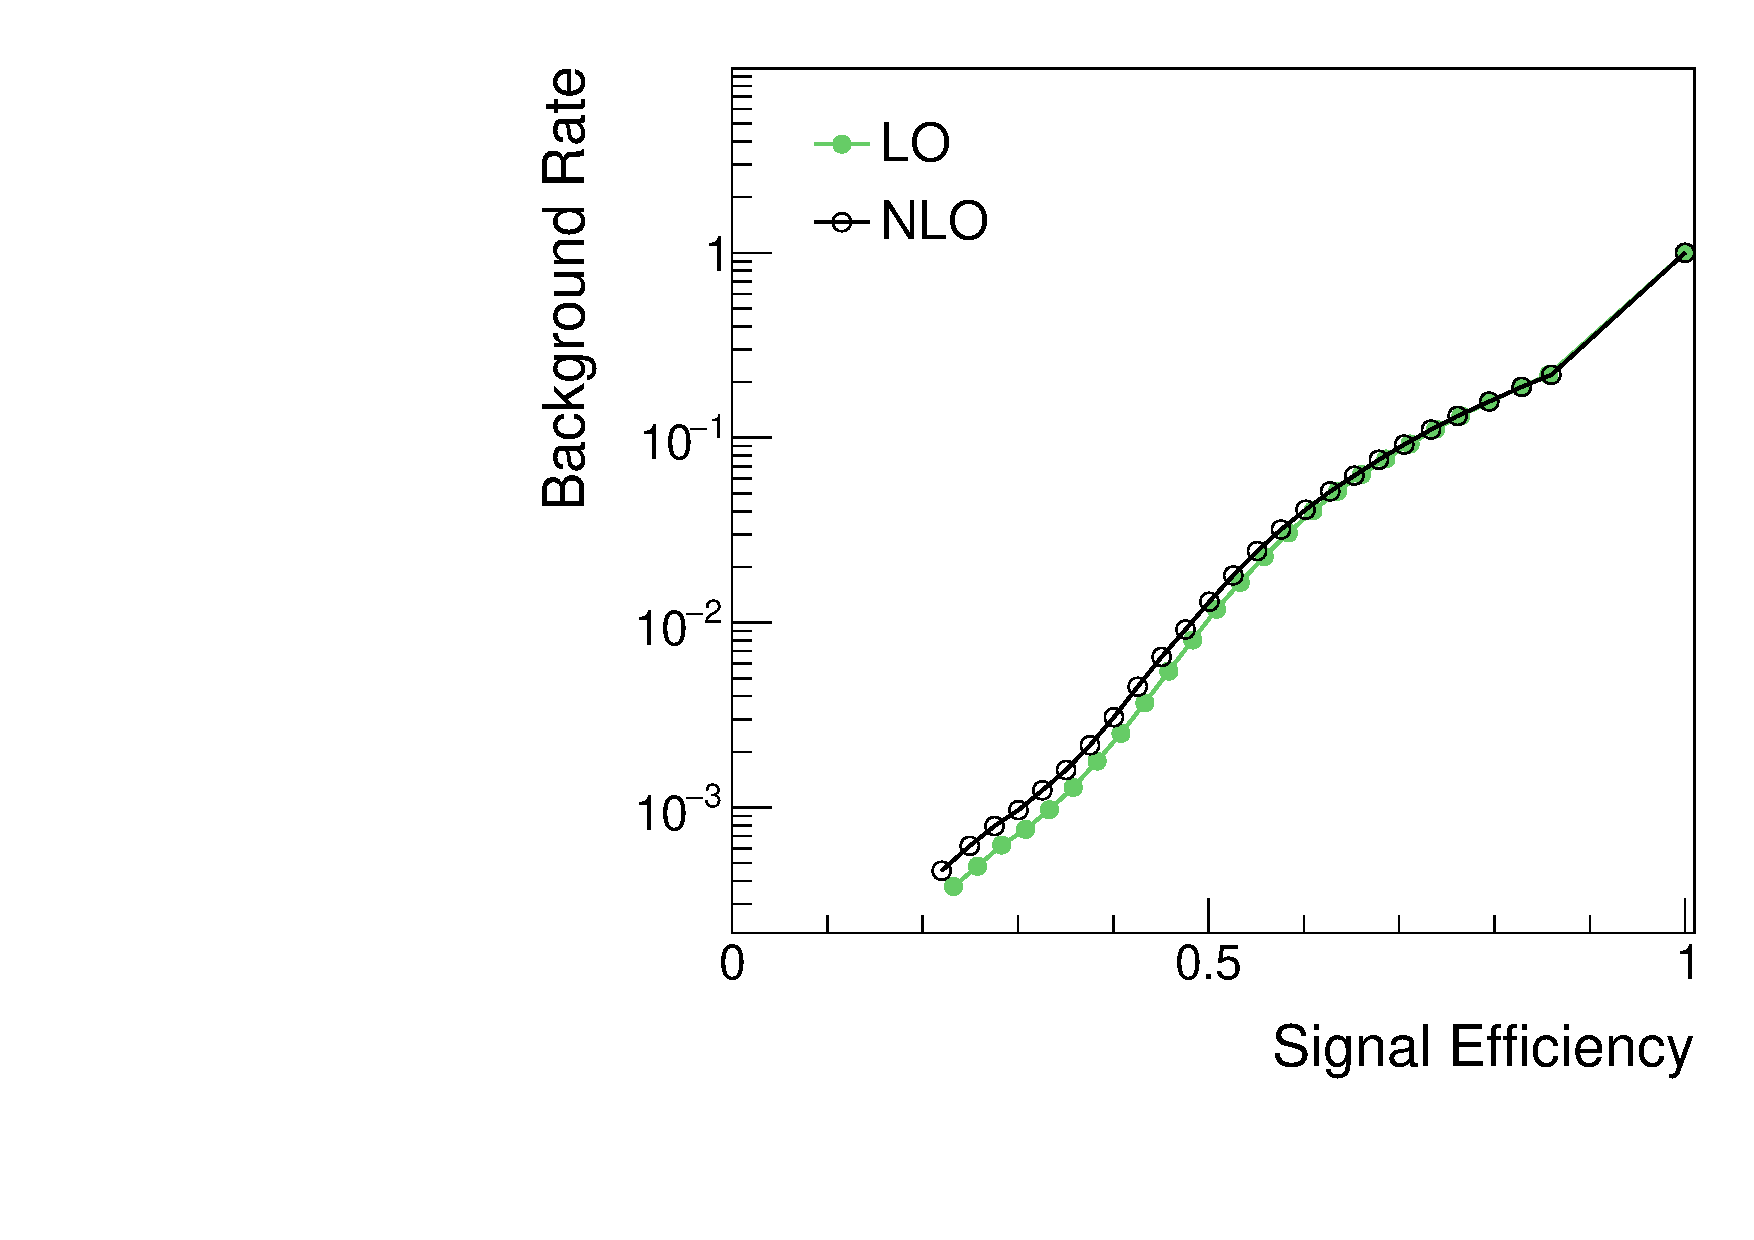
\includegraphics[width=0.57\textwidth]{plots/hh_bbwwMEM_dilepton_lo_vs_nlo_ROC.pdf}
\fi
\caption{
  Separation between the $\dihiggs$ signal and the $\ttbar$ background 
  for events simulated at LO and at NLO accuracy in pQCD.
  The graphs of background rate versus signal efficiency shown in the figure
  are obtained by applying a cut on the distributions in the likelihood ratios $P(\vecy)$ shown in Fig.~\ref{fig:memLR_LO_vs_NLO}.
}
\label{fig:ROC_LO_vs_NLO}
\end{figure}

The computing time required to evaluate the integrals given by Eqs.~(\ref{eq:mem_signal}) and~(\ref{eq:mem_background})
may represent a challenge in practical applications of the MEM.
Experimental analyses will usually need to evaluate these integrals
multiple times for each event in order to assess the effect of systematic uncertainties.
Taken together with the large cross section for $\ttbar$ production at the LHC,
the integrals in Eqs.~(\ref{eq:mem_signal}) and~(\ref{eq:mem_background}) may need to be computed in the order of $100$ million times.
Even with several thousands of computing jobs running in parallel,
as it is nowadays commonplace for experimental data analyses performed at the LHC,
the computation still requires a few weeks of nonstop computing time.
Several possibilities to speed up the numeric integrations, which take most of the computing time in practical applications of the MEM,
have been explored in the literature.
One alternative is to use vector integrands to evaluate the likelihood ratio for all systematic uncertainties simultaneously~\cite{CUBA},
taking advantage of the fact that the systematic uncertainties typically constitute small changes with respect to the nominal value.
Another alternative is to take advantage of the parallelizability of multidimensional integration and perform the integration on graphics processing units (GPUs).
Speedup factors of order $100$, compared to using a single core of a general-purpose central processing unit (CPU) 
such as the $2.30$~GHz Intel\TReg~Xeon\TReg~E5-2695V3 processor that we used for the studies presented in this paper,
are reported in the literature for performing numeric integrations on GPUs~\cite{Hagiwara:2009aq,Hagiwara:2009cy,Kanzaki:2010ym,Hagiwara:2013oka,Schouten:2014yza,Grasseau:2015vfa}.
